%!TEX TS-program = xelatex

% Заготовка презентации по проекту.
% Основано на шаблоне presentation/example-beamer-HSE-ru.tex.

\documentclass[aspectratio=169]{beamer}

\newbool{russian}
\booltrue{russian}
\usepackage{graphicx}
\usepackage{HSE-theme/beamerthemeHSE}

%%% Работа с русским языком и шрифтами
\usepackage[english,russian]{babel}
\usepackage[no-math]{fontspec}
\IfFontExistsTF{HSE Sans}{%
    \setsansfont{HSE Sans}%
    \setmainfont{HSE Sans}%
}{%
    \setsansfont{Arial}%
    \setmainfont{Arial}%
}
\setmonofont{Courier New}
\usepackage{bookmark}
\uselanguage{russian}
\languagepath{russian}
\deftranslation[to=russian]{Theorem}{Теорема}
\deftranslation[to=russian]{Definition}{Определение}
\deftranslation[to=russian]{Definitions}{Определения}
\deftranslation[to=russian]{Corollary}{Следствие}
\deftranslation[to=russian]{Fact}{Факт}
\deftranslation[to=russian]{Example}{Пример}
\deftranslation[to=russian]{Examples}{Примеры}

%%% Дополнительные пакеты для рабочих слайдов
\usepackage{booktabs}
\usepackage{array}

%%% Пути к изображениям
\graphicspath{{images/}{../figures/output/}{figures/output/}}

%%% Информация об авторе и выступлении
\title[ДКП и рецессии]{Генерирует ли денежно-кредитная политика рецессии?}
\subtitle{Структурная идентификация шоков денежно-кредитной политики}

\author[Поздняков М. А.]{Поздняков Михаил Александрович}

\institute{Факультет экономических наук\\НИУ ВШЭ}

\date{Москва, 2026}

\begin{document}

% Заглавный слайд
\frame[plain,noframenumbering]{\titlepage}


\section{Исходная статья}
\begin{frame}{Исследовательский вопрос}
\small
\begin{itemize}
\setlength\itemsep{0.45em}
\item Статья Sims--Zha отвечает на вопрос: генерирует ли денежно-кредитная политика рецессии?
\item Этот вопрос требует отделить собственно шоки политики от систематической реакции центрального банка на состояние экономики.
\item Поэтому центральная эмпирическая проблема статьи — идентификация монетарных шоков в структурной VAR-модели.
\end{itemize}
\end{frame}

\begin{frame}{Эмпирические аномалии как проблема идентификации}
\small
\begin{itemize}
\setlength\itemsep{0.5em}
\item Инновации денежной массы и процентной ставки не всегда дают теоретически ожидаемые реакции выпуска, цен и ставок.
\item Это проявляется в двух известных аномалиях: «загадке ликвидности» и «загадке цен».
\item Следовательно, нужен переход от приведённой VAR к структурной модели с явными ограничениями.
\end{itemize}
\end{frame}
\begin{frame}{Допустимость VAR}
\small
\begin{itemize}
\setlength\itemsep{0.5em}
\item В реальной экономике шоков больше, чем переменных в моделях
\item Способность VAR восстанавливать монетарный шок проверяется с помощью DSGE
\item Но этот результат зависит от включения ключевых информационных переменных (отражающих ожидания и инфляционные сигналы)
\end{itemize}
\end{frame}

\begin{frame}[t]{SVAR-модель Sims--Zha}
\small

Sims--Zha используют \textbf{структурную VAR-модель}: приведённая VAR описывает динамику данных, а структурная форма нужна для интерпретации шоков.

\vspace{0.35em}

\begin{columns}[T,onlytextwidth]

\begin{column}{0.48\textwidth}
\textbf{Вектор переменных}

\vspace{0.3em}

\begin{itemize}
\setlength\itemsep{0.32em}
\item \textbf{Денежный блок:} $R$ — краткосрочная ставка; $M$ — M2 или совокупные резервы.
\item \textbf{Реальная экономика:} $y$ — выпуск; $W$ — заработная плата.
\item \textbf{Цены:} $P_y$ — дефлятор выпуска; $P_{im}$ — цены промежуточных материалов.
\item \textbf{Информационные переменные:} $Tbk$ — банкротства; $P_{cm}$ — сырьевые цены.
\end{itemize}

\vspace{0.25em}

\footnotesize
Идентификация задаётся ограничениями на $\Gamma_0$.
\end{column}

\begin{column}{0.48\textwidth}
\textbf{Структурная и приведённая формы}

\vspace{0.25em}

\footnotesize

$$
\Gamma(L)y_t = \varepsilon_t
$$

$$
[I - B(L)]y_t = u_t
$$

$$
I - B(L) = \Gamma_0^{-1}\Gamma(L)
$$

$$
\Gamma_0 \Sigma_u \Gamma_0' = \Lambda
$$

\vspace{0.15em}

Здесь $\varepsilon_t$ — структурные шоки, $u_t$ — остатки приведённой VAR, $\Lambda$ — диагональная ковариационная матрица структурных шоков.
\end{column}

\end{columns}

\end{frame}
\begin{frame}[t]{Матрица идентификации: M2-модель}
\footnotesize

Идентификация задаётся ограничениями на матрицу одновременных связей $\Gamma_0$.
Строки соответствуют уравнениям структурных шоков, столбцы --- текущим переменным.

\vspace{0.35em}

\begin{center}
\scriptsize
\setlength{\tabcolsep}{2.8pt}
\renewcommand{\arraystretch}{1.15}

\begin{tabular}{@{}lrrrrrrrr@{}}
\toprule
Шок / уравнение & $P_{cm}$ & $M$ & $R$ & $P_{im}$ & $P_y$ & $W$ & $y$ & $Tbk$ \tabularnewline
\midrule
$P_{cm}$ & 1.91 & -200.87 & -7.98 & -21.05 & -206.11 & 111.96 & -53.87 & -10.91 \tabularnewline
$MD$     & 0 & 150.23 & 77.94 & 0 & -150.23 & 0 & -150.23 & 0 \tabularnewline
$MS$     & -11.93 & 10.33 & 182.42 & 0 & 0 & 0 & 0 & 36.95 \tabularnewline
$P_{im}$ & -24.97 & 0 & 0 & 178.26 & -81.95 & -127.61 & 7.92 & 13.97 \tabularnewline
$P_y$    & -4.07 & 0 & 0 & 0 & 433.74 & -287.44 & -56.18 & -26.70 \tabularnewline
$W$      & 1.00 & 0 & 0 & 0 & 0 & -435.81 & 113.33 & -0.04 \tabularnewline
$y$      & -13.89 & 0 & 0 & 0 & 0 & 0 & 27.30 & -77.19 \tabularnewline
$Tbk$    & 33.97 & 0 & 0 & 0 & 0 & 0 & 0 & -40.18 \tabularnewline
\bottomrule
\end{tabular}
\end{center}

\vspace{0.35em}

\footnotesize
$MD$ --- шок спроса на деньги, $MS$ --- шок денежной политики. В M2-модели уравнение $MS$ допускает текущую реакцию на $Tbk$.

\end{frame}

\begin{frame}[t]{Матрица идентификации: TR-модель}
\footnotesize

TR-спецификация сохраняет ту же общую структуру ограничений, но меняет уравнение денежной политики.

\vspace{0.35em}

\begin{center}
\scriptsize
\setlength{\tabcolsep}{2.8pt}
\renewcommand{\arraystretch}{1.15}

\begin{tabular}{@{}lrrrrrrrr@{}}
\toprule
Шок / уравнение & $P_{cm}$ & $M$ & $R$ & $P_{im}$ & $P_y$ & $W$ & $y$ & $Tbk$ \tabularnewline
\midrule
$P_{cm}$ & 13.14 & -6.01 & -49.56 & 30.23 & -67.06 & 156.60 & 30.04 & -66.36 \tabularnewline
$MD$     & 0 & 25.01 & 124.25 & 0 & -25.01 & 0 & -25.01 & 0 \tabularnewline
$MS$     & -4.14 & -99.76 & 51.96 & 0 & 0 & 0 & 0 & 0 \tabularnewline
$P_{im}$ & -26.29 & 0 & 0 & 173.25 & -79.14 & -120.80 & 0.51 & 23.95 \tabularnewline
$P_y$    & -2.34 & 0 & 0 & 0 & 490.42 & -238.21 & 14.19 & -24.18 \tabularnewline
$W$      & -6.67 & 0 & 0 & 0 & 0 & 412.96 & -82.62 & 28.65 \tabularnewline
$y$      & -6.92 & 0 & 0 & 0 & 0 & 0 & 168.90 & 33.61 \tabularnewline
$Tbk$    & 31.22 & 0 & 0 & 0 & 0 & 0 & 0 & 39.65 \tabularnewline
\bottomrule
\end{tabular}
\end{center}

\vspace{0.35em}

\footnotesize
Главное отличие от M2-модели: в строке $MS$ коэффициент при $Tbk$ равен нулю, то есть политика не реагирует на банкротства внутри квартала.

\end{frame}

\begin{frame}[t]{Основные результаты Sims--Zha}
\small

\vspace{0.3em}

\begin{columns}[T,onlytextwidth]

\begin{column}{0.31\textwidth}
\textbf{Импульсные отклики}

\vspace{0.3em}
\footnotesize
Идентифицированные монетарные шоки дают осмысленные реакции переменных, но эффект на выпуск ограничен.
\end{column}

\begin{column}{0.31\textwidth}
\textbf{Историческая декомпозиция}

\vspace{0.3em}
\footnotesize
Неожиданные сдвиги политики не объясняют основную часть исторических рецессий.
\end{column}

\begin{column}{0.31\textwidth}
\textbf{Контрфакты}

\vspace{0.3em}
\footnotesize
Правила с фиксированными $M$ или $R$ не дают существенного сглаживания делового цикла.
\end{column}

\end{columns}

\vspace{1.0em}

\begin{block}{Главный вывод}
\small
Рецессии в основном не являются следствием автономных монетарных шоков; важнее систематическая реакция политики на состояние экономики.
\end{block}

\end{frame}


\section{Российская адаптация}
\begin{frame}{Переход к российской спецификации}

\textbf{Вопрос:} можно ли на российских квартальных данных получить
интерпретируемую VAR/SVAR-модель денежно-кредитной трансмиссии по мотивам Sims---Zha?

\vspace{0.4cm}

\begin{itemize}
    \item Исходная статья: США, квартальные данные, роль шоков ДКП.
    \item Наша задача: адаптация логики модели.
    \item Причина: другая денежно-кредитная система и другой набор доступных рядов.
    \item Общая идея спецификации сохраняется, набор переменных адаптируется
\end{itemize}

\end{frame}
\begin{frame}{Используемые переменные}

\scriptsize
\setlength{\tabcolsep}{5pt}
\renewcommand{\arraystretch}{1.35}

\begin{tabular}{p{2.6cm} p{3.0cm} p{4.7cm}}
\hline
\textbf{Блок} & \textbf{Переменные} & \textbf{Роль в модели} \\
\hline

Сырьевые цены
& $\log P_{cm,t}$
& Быстрый индикатор инфляционного давления. \\

Денежно-кредитный блок
& $\log M2_t$, $R_t$
& Денежная масса и ключевая ставка Банка России. \\

Промежуточные цены
& $\log P_{im,t}$
& Канал производственных издержек. \\

Цены и доходы
& $\log P_t$, $\log W_t$
& ИПЦ и реальная заработная плата. \\

Реальный сектор
& $\log Y_t$
& Реальный ВВП. \\

Финансовый стресс
& $\log OvDeb_t$
& Просроченная задолженность; аналог банкротств. \\
\hline
\end{tabular}

\vspace{0.25cm}

{\tiny Источники данных: Банк России, Росстат, ЕМИСС, ИЭП им. Е. Т. Гайдара; расчёты автора.}

\end{frame}
\begin{frame}{Подготовка данных}

\begin{itemize}
    \item Базовая выборка начинается с 2014 года: после перехода Банка России
    к режиму инфляционного таргетирования.

    \item Все ряды приведены к квартальной частоте.

    \item Если сезонно скорректированный ряд доступен в источнике, используется он;
    иначе применяется X-13ARIMA-SEATS.

    \item Уровневые переменные логарифмируются; ключевая ставка используется
    в процентных пунктах без логарифмирования.

    \item Отдельно построены российские аналоги переменных Sims--Zha:
    сырьевой индекс, индекс промежуточных материалов и показатель финансового стресса.
\end{itemize}

\vspace{0.2cm}

{\scriptsize Источники: Банк России, Росстат, ЕМИСС, ИЭП им. Е. Т. Гайдара; расчёты автора.}

\end{frame}
\begin{frame}[t]{Российская структурная идентификация}

\scriptsize
\centering

\[
\hat A X_t = A_1 X_{t-1} + \varepsilon_t
\]

\vspace{-0.15cm}

\resizebox{\textwidth}{!}{%
\begin{tabular}{lrrrrrrrr}
\toprule
Уравнение & $P_{cm}$ & $M2$ & $R$ & $P_{im}$ & $P_y$ & $W$ & $y$ & $OvDeb$ \\
\midrule
$P_{cm}$ & $-6.11$ & $109.58$ & $0.29$ & $10.84$ & $-215.24$ & $-103.17$ & $80.94$ & $8.75$ \\
$MD$     & $0$     & $46.05$  & $0.59$ & $0$     & $-46.05$  & $0$       & $-46.05$ & $0$ \\
$MS$     & $-0.05$ & $-111.76$ & $0.39$ & $0$     & $0$       & $0$       & $0$      & $-1.46$ \\
$P_{im}$ & $-20.00$& $0$      & $0$    & $43.17$ & $-63.60$  & $4.50$    & $-16.46$ & $-5.15$ \\
$P_y$    & $2.01$  & $0$      & $0$    & $0$     & $-149.70$ & $-33.47$  & $-45.78$ & $10.10$ \\
$W$      & $6.78$  & $0$      & $0$    & $0$     & $0$       & $74.13$   & $-42.96$ & $10.04$ \\
$y$      & $14.02$ & $0$      & $0$    & $0$     & $0$       & $0$       & $-48.32$ & $4.25$ \\
$OvDeb$  & $-1.83$ & $0$      & $0$    & $0$     & $0$       & $0$       & $0$      & $26.03$ \\
\bottomrule
\end{tabular}
}

\vspace{0.2cm}

\begin{itemize}
    \item Нули задают ограничения на текущие связи внутри квартала.
    \item $MD$ --- денежный спрос; $MS$ --- денежно-кредитная политика.
    \item $P_{cm}$ может реагировать быстро; остальные частные переменные образуют более инерционный блок.
\end{itemize}

\end{frame}

\section{Результаты}
\begin{frame}[t]{Функции импульсного отклика}

\vspace{-0.25cm}

\begin{columns}[T,totalwidth=\textwidth]

\begin{column}{0.76\textwidth}
\centering
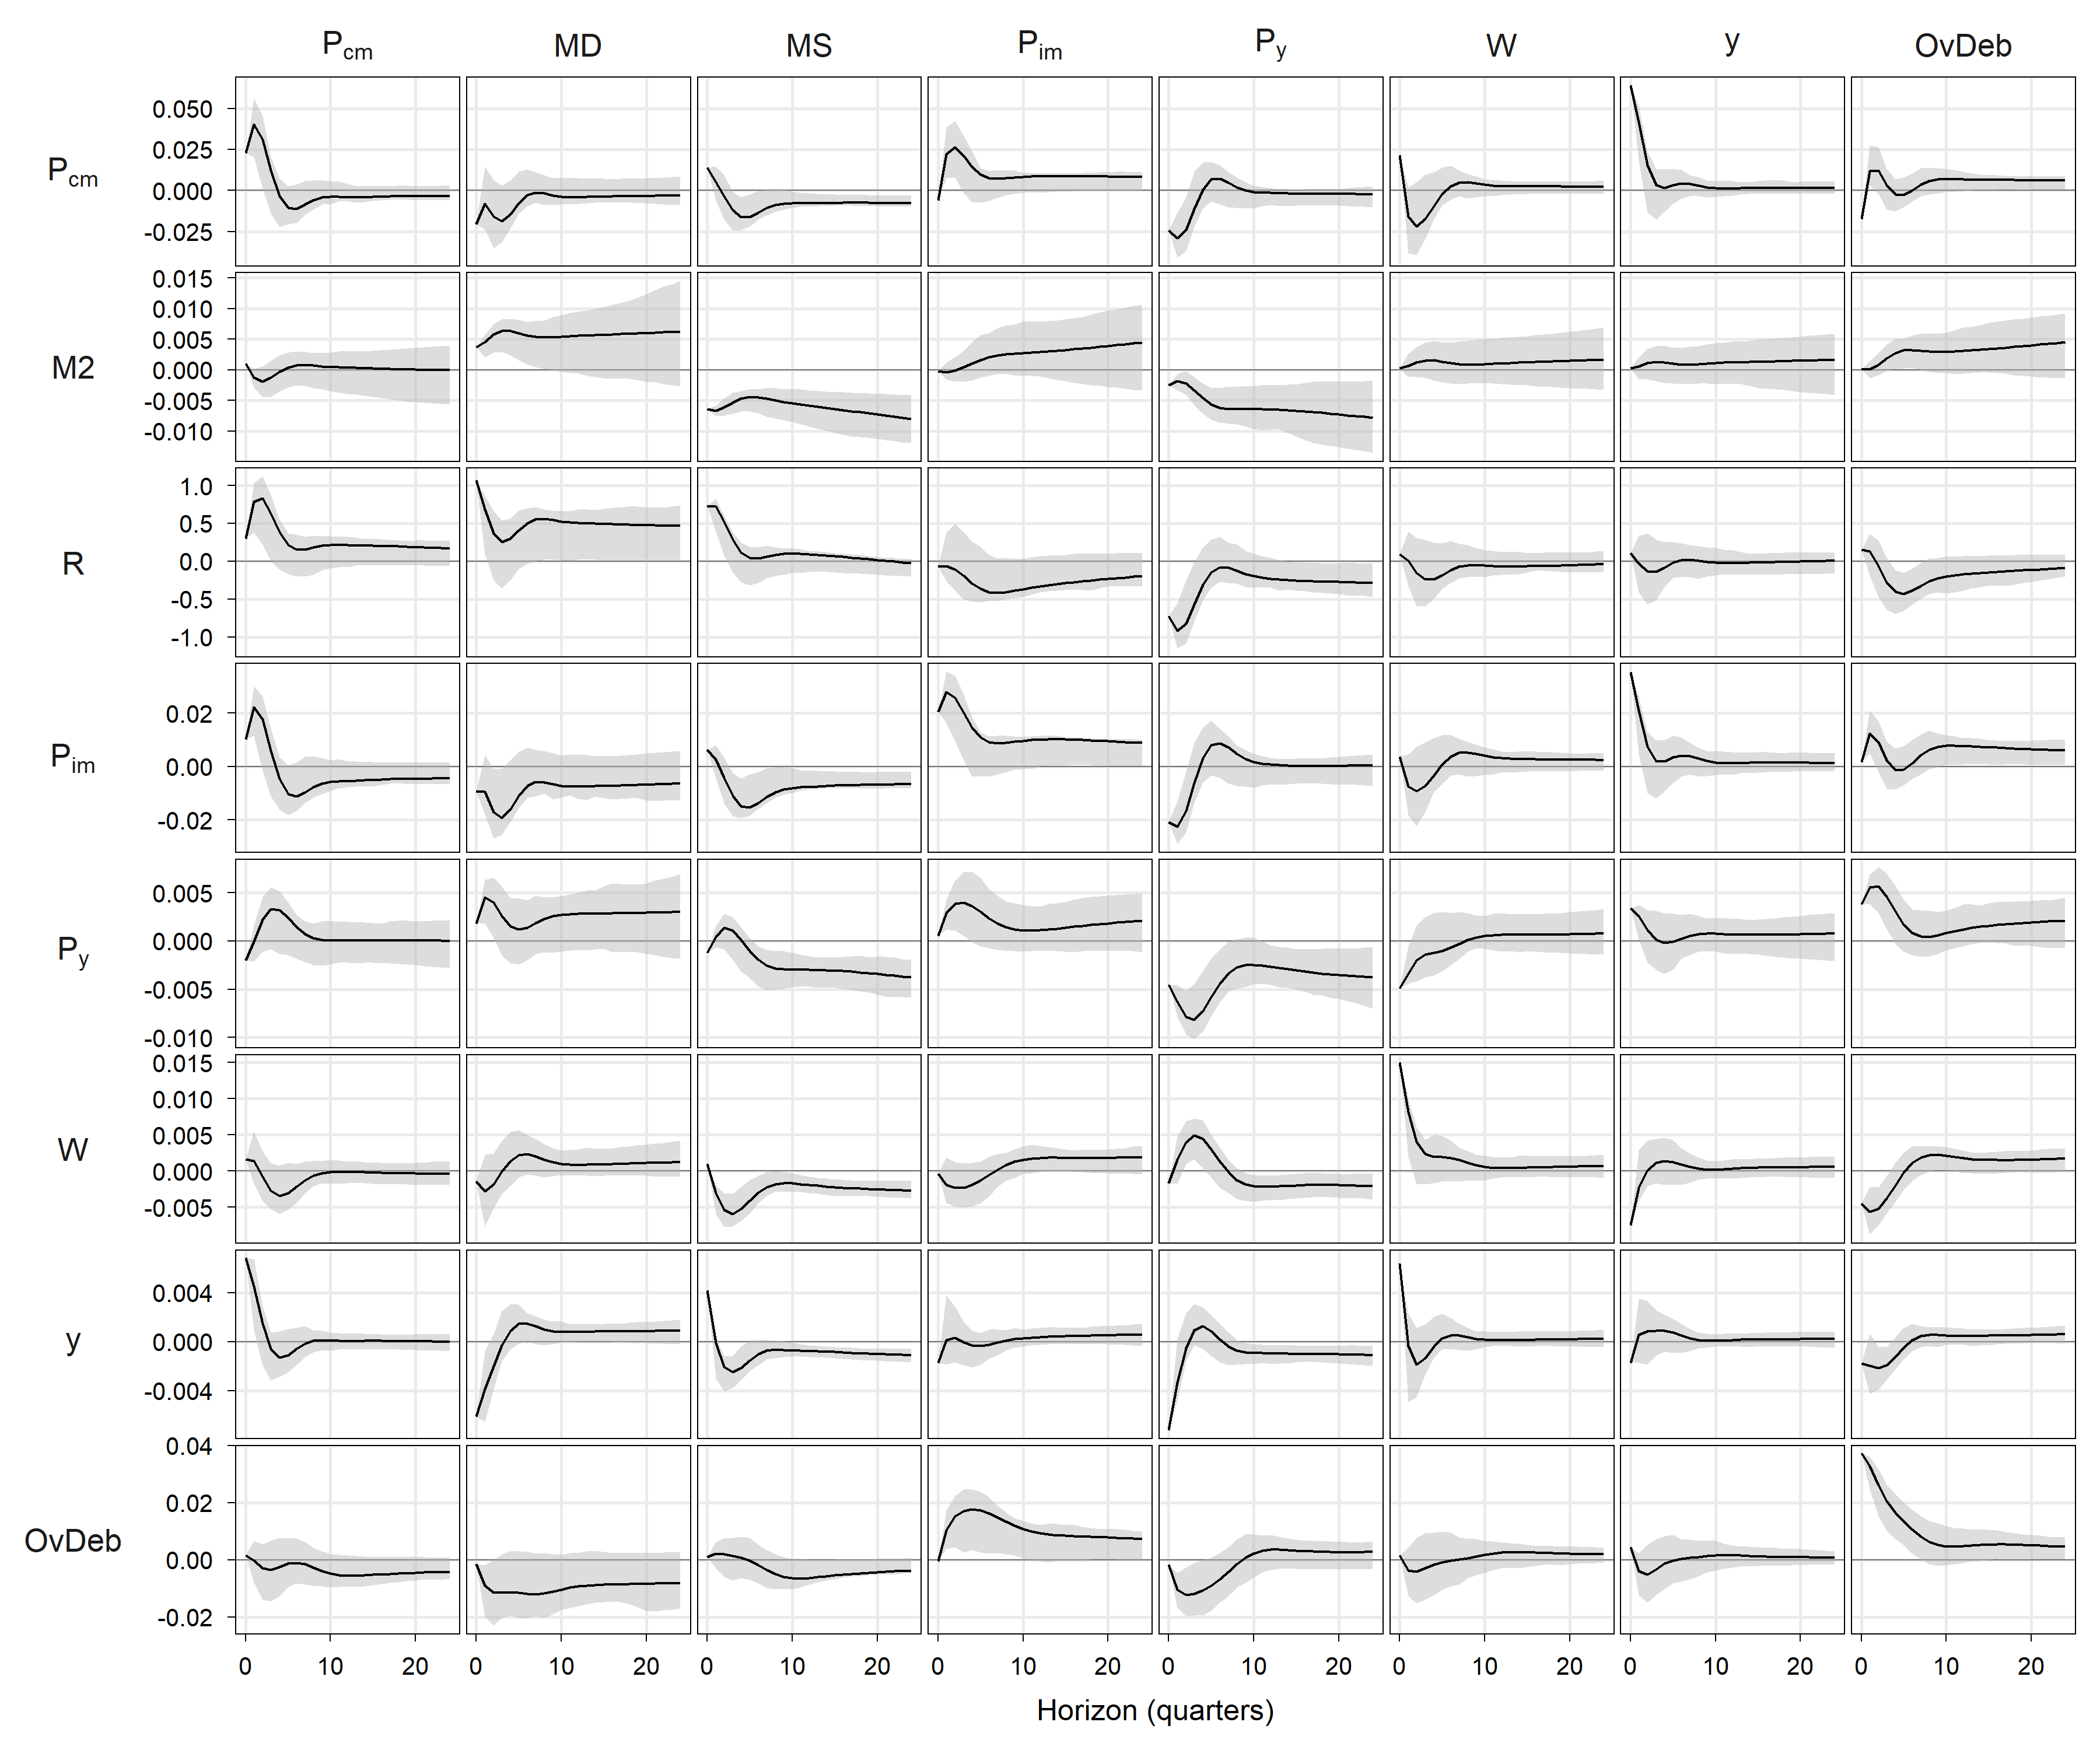
\includegraphics[
    width=\linewidth,
    height=0.84\textheight,
    keepaspectratio
]{irf_full_grid_presentation.png}
\end{column}

\begin{column}{0.22\textwidth}
\scriptsize

\textbf{Как читать график}

\vspace{0.15cm}

\begin{itemize}
    \item строки --- реагирующие переменные;
    \item столбцы --- структурные шоки;
    \item основной интерес: $MS$ и $MD$.
\end{itemize}

\vspace{0.2cm}

\textbf{Интерпретация}

\vspace{0.15cm}

Шок $MS$ соответствует ужесточению ДКП: ставка растёт, $M2$ снижается, выпуск и цены затем ослабевают.

\end{column}

\end{columns}

\end{frame}
\begin{frame}[t]{Историческая декомпозиция: денежный блок}

\vspace{-0.25cm}

\begin{center}
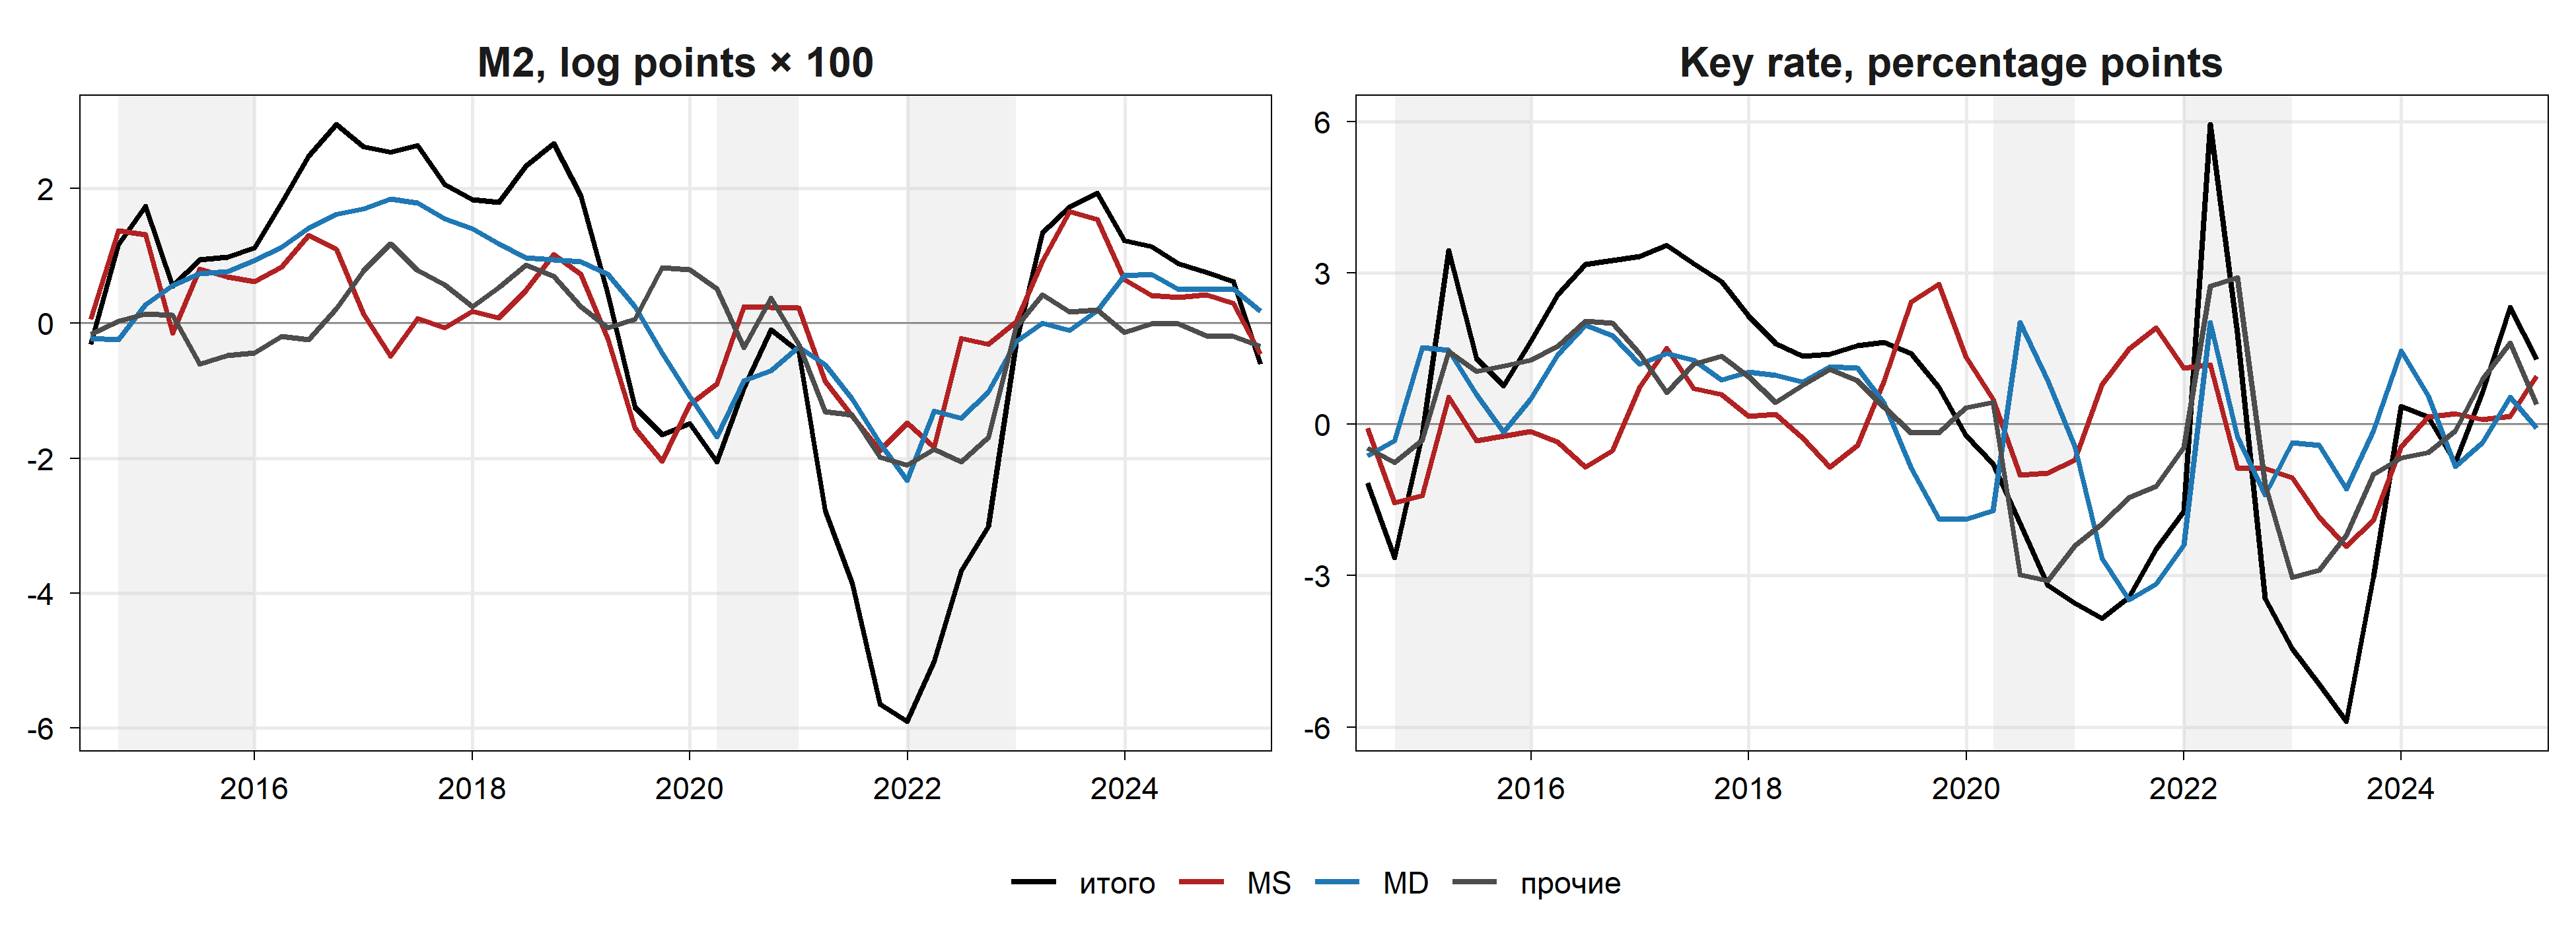
\includegraphics[
    width=\textwidth,
    height=0.78\textheight,
    keepaspectratio
]{hd_money_block_compact.png}
\end{center}

\vspace{-0.1cm}

{\scriptsize
Движение $M2$ и $R$ не сводится к шоку денежно-кредитной политики $MS$:
заметны вклад денежного спроса $MD$ и неденежных шоков.
}

\end{frame}
\begin{frame}[t]{Историческая декомпозиция: цены и выпуск}

\vspace{-0.25cm}

\begin{center}
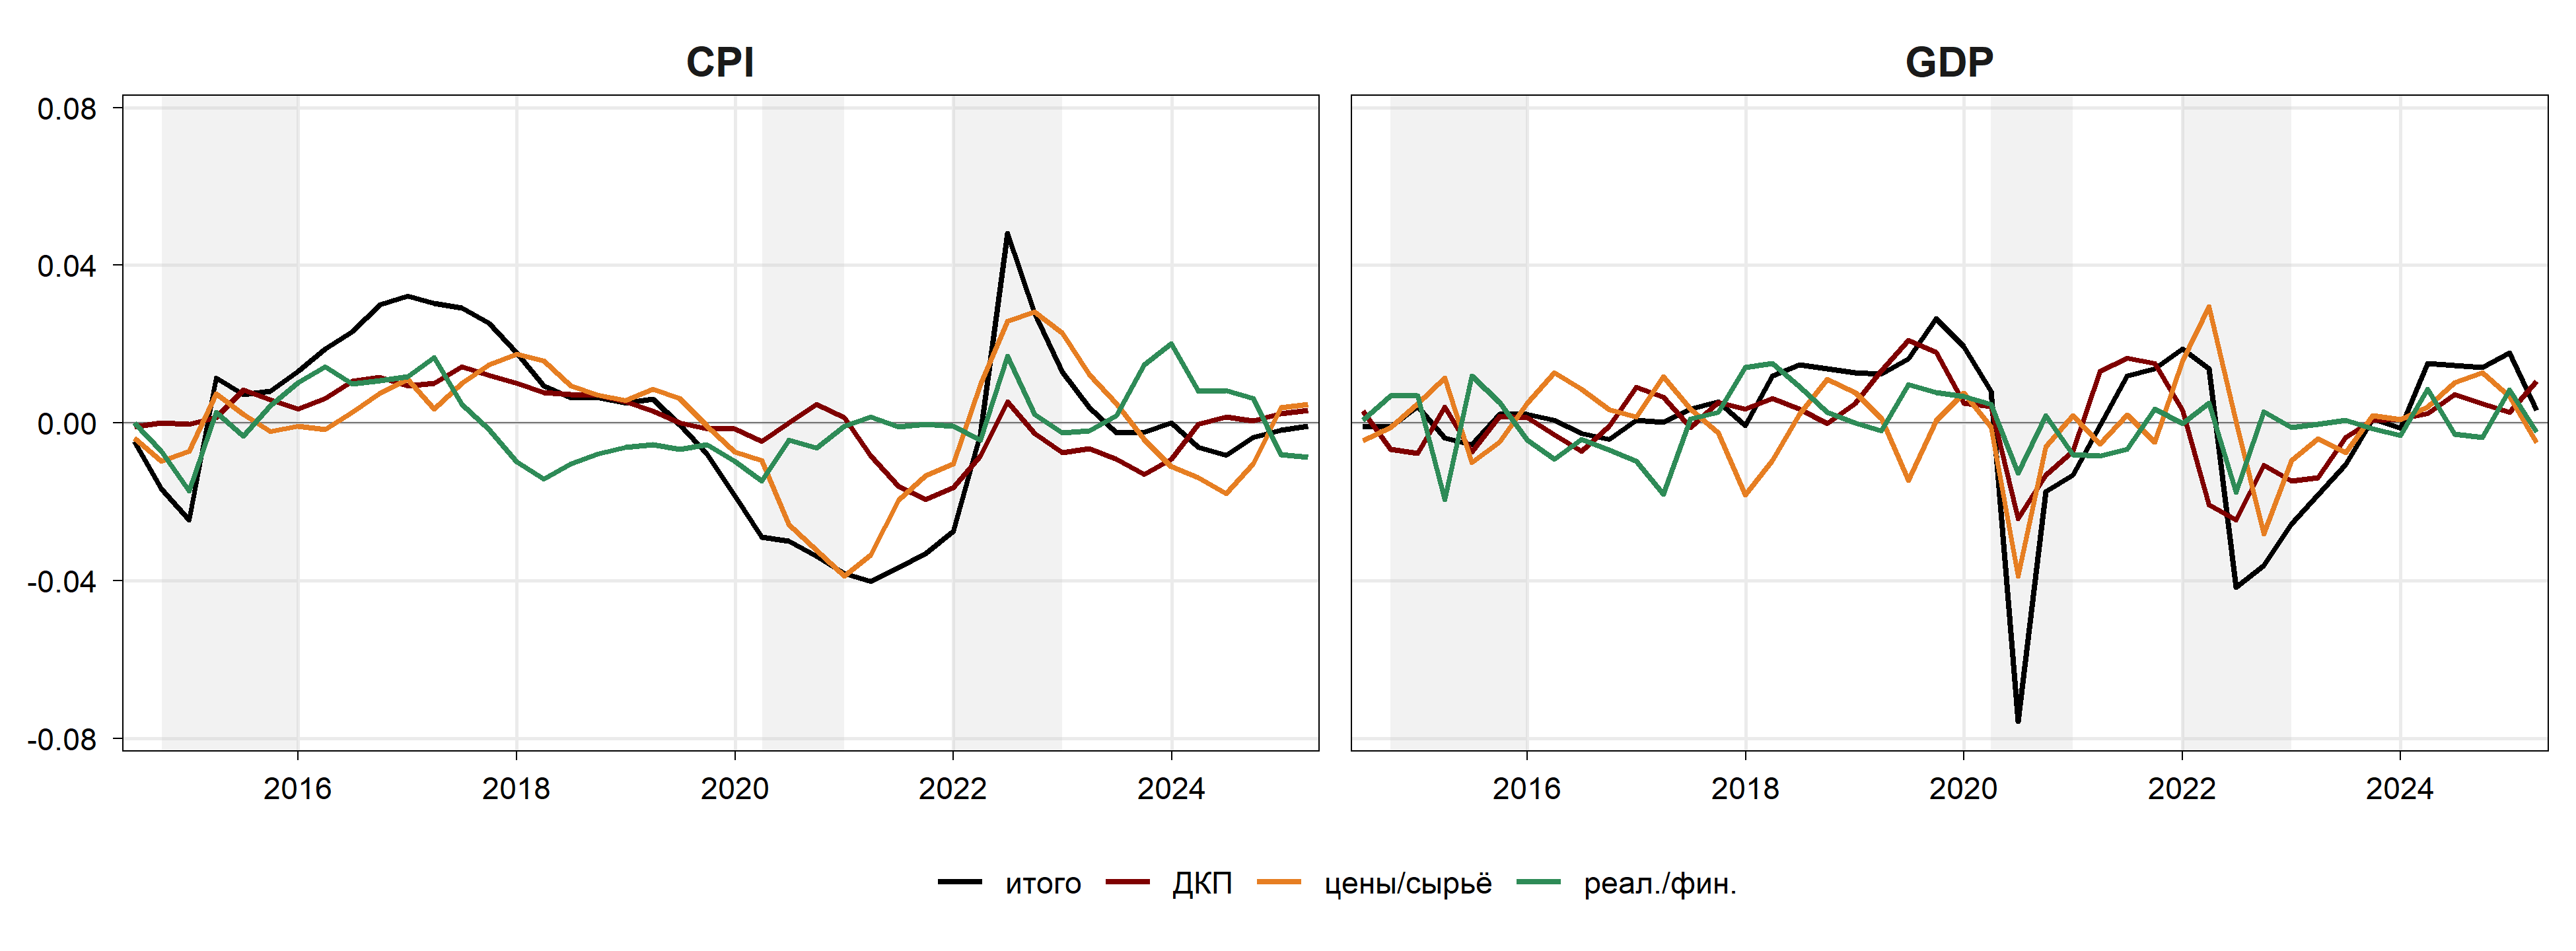
\includegraphics[
    width=\textwidth,
    height=0.78\textheight,
    keepaspectratio
]{hd_prices_output_compact.png}
\end{center}

\vspace{-0.1cm}

{\scriptsize
Колебания цен и выпуска не объясняются только автономными шоками ДКП:
важны ценовые, сырьевые, реальные и финансовые компоненты.
}

\end{frame}
\begin{frame}[t]{Альтернативная политика: фиксированная ставка}

\vspace{-0.25cm}

\begin{center}
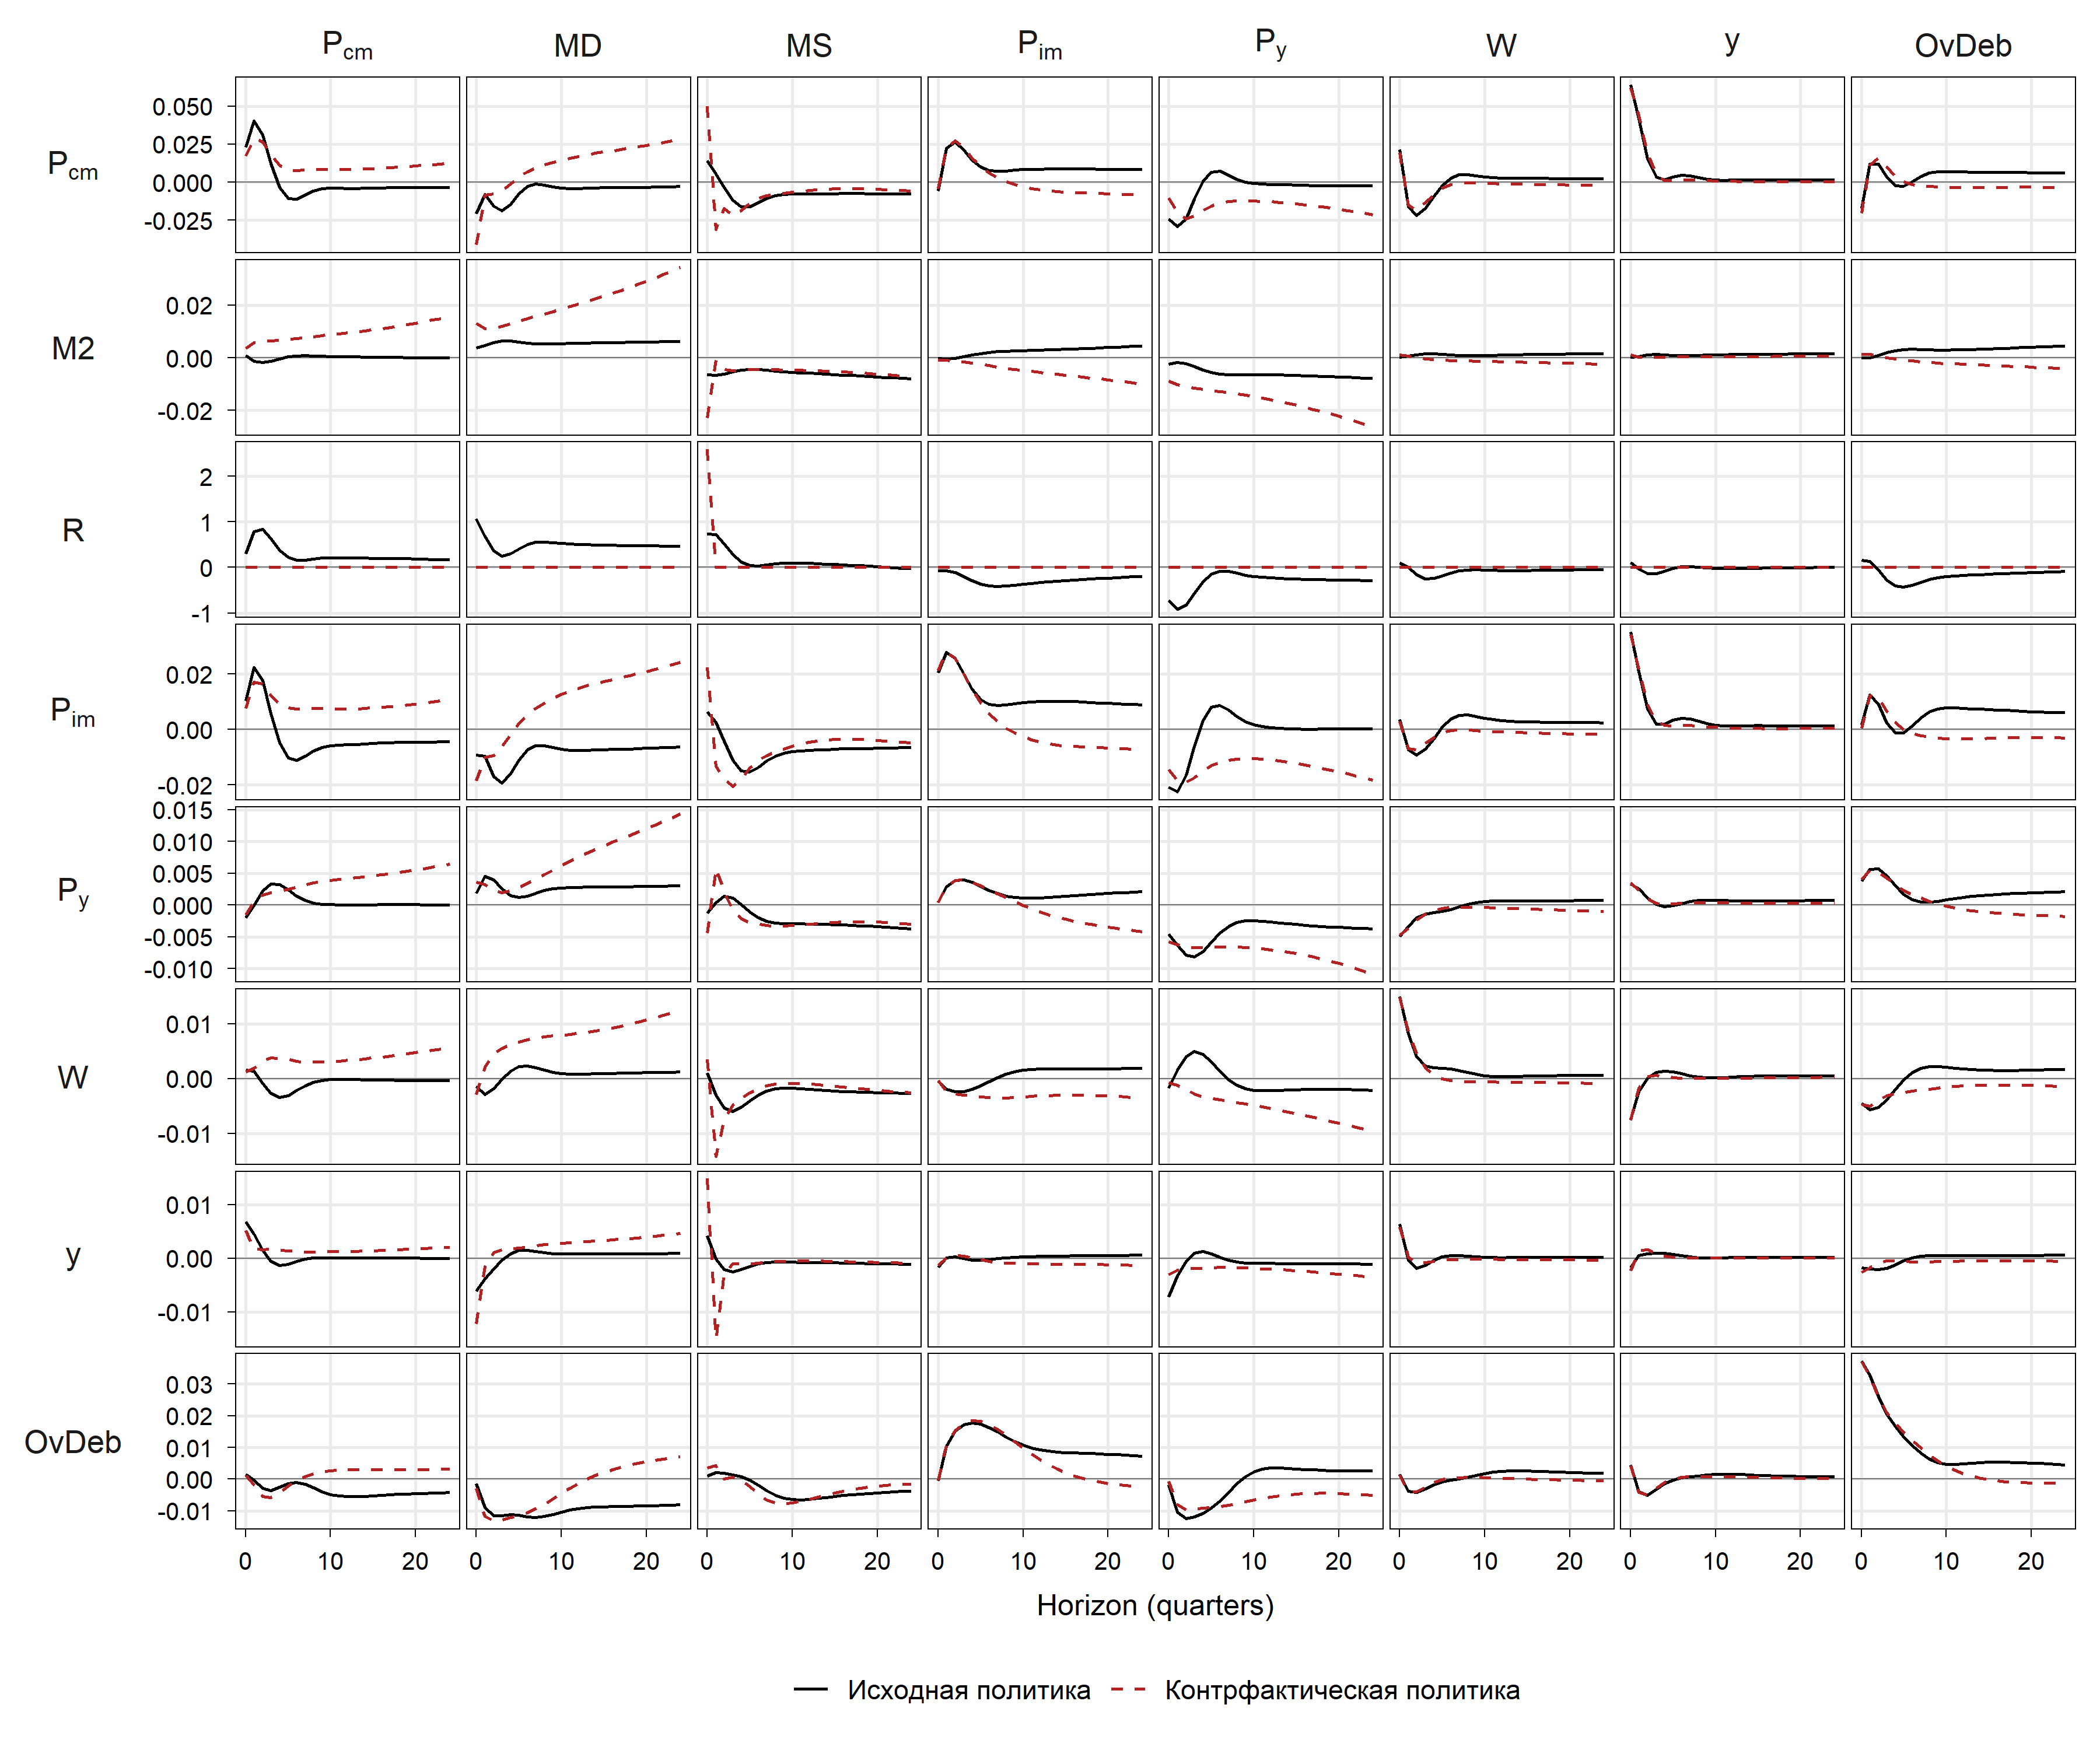
\includegraphics[
    width=\textwidth,
    height=0.78\textheight,
    keepaspectratio
]{policy_fixed_key_rate_presentation.png}
\end{center}

\vspace{-0.1cm}

{\scriptsize
Контрфакт показывает, как изменилась бы динамика ключевых переменных,
если бы траектория ключевой ставки была зафиксирована.
}

\end{frame}


\begin{frame}[t]{Альтернативная политика: фиксированный M2}

\vspace{-0.25cm}

\begin{center}
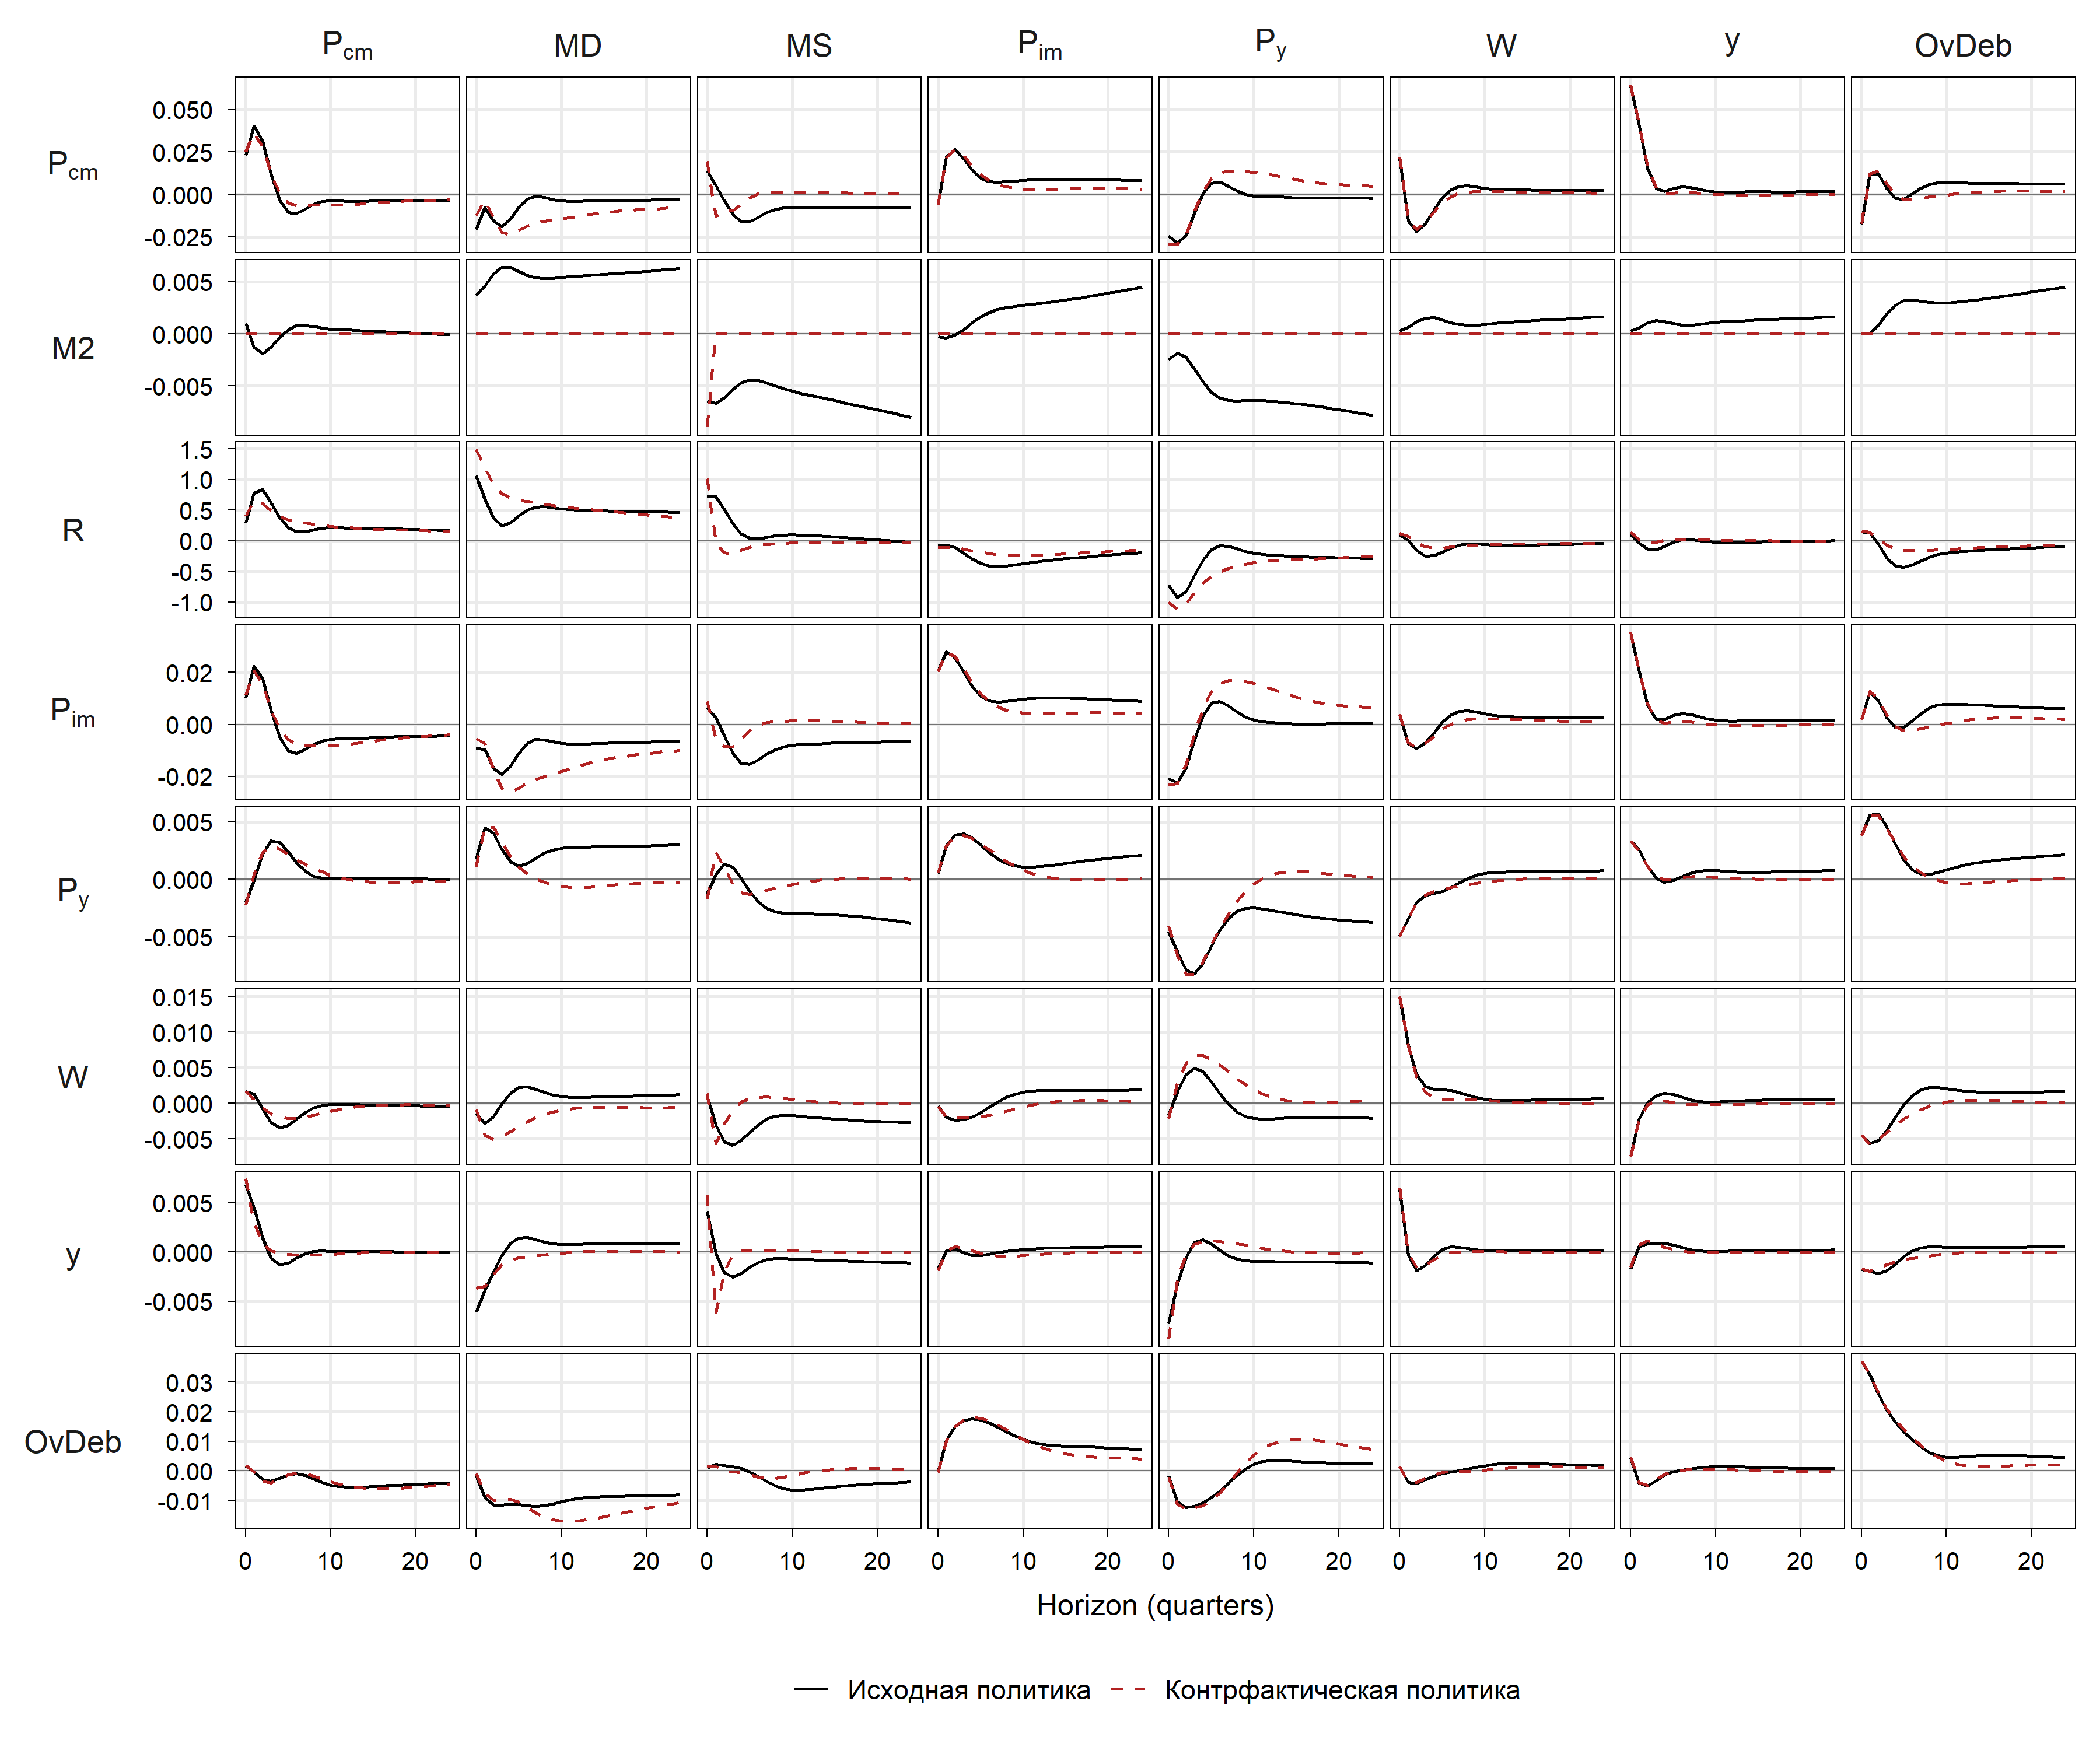
\includegraphics[
    width=\textwidth,
    height=0.78\textheight,
    keepaspectratio
]{policy_fixed_m2_presentation.png}
\end{center}

\vspace{-0.1cm}

{\scriptsize
Контрфакт показывает, как изменилась бы динамика ключевых переменных,
если бы траектория денежного агрегата $M2$ была зафиксирована.
}

\end{frame}
\begin{frame}{Вывод}

\begin{itemize}
    \item Российская SVAR-модель даёт интерпретируемые шоки ДКП.

    \item Реакции денежного блока согласуются с экономической логикой:
    $MS$ повышает ставку и снижает $M2$.

    \item Кризисы 2014--2015, 2020 и 2022 годов не сводятся к автономным
    шокам ДКП.

    \item Фиксация $R$ или $M2$ не устраняет основные колебания цен и выпуска.
\end{itemize}

\vspace{0.25cm}

\textbf{Итог:} ДКП в основном реагируют на кризисы, а не порождают спады.

\end{frame}


% Повтор заглавного слайда в конце презентации
\frame[plain,noframenumbering]{\titlepage}


{
\setbeamertemplate{footline}{}
\appendix
\section{Приложение}

\begin{frame}[t,noframenumbering]{Приложение: историческая декомпозиция $M2$}
\vspace{-0.25cm}
\centering
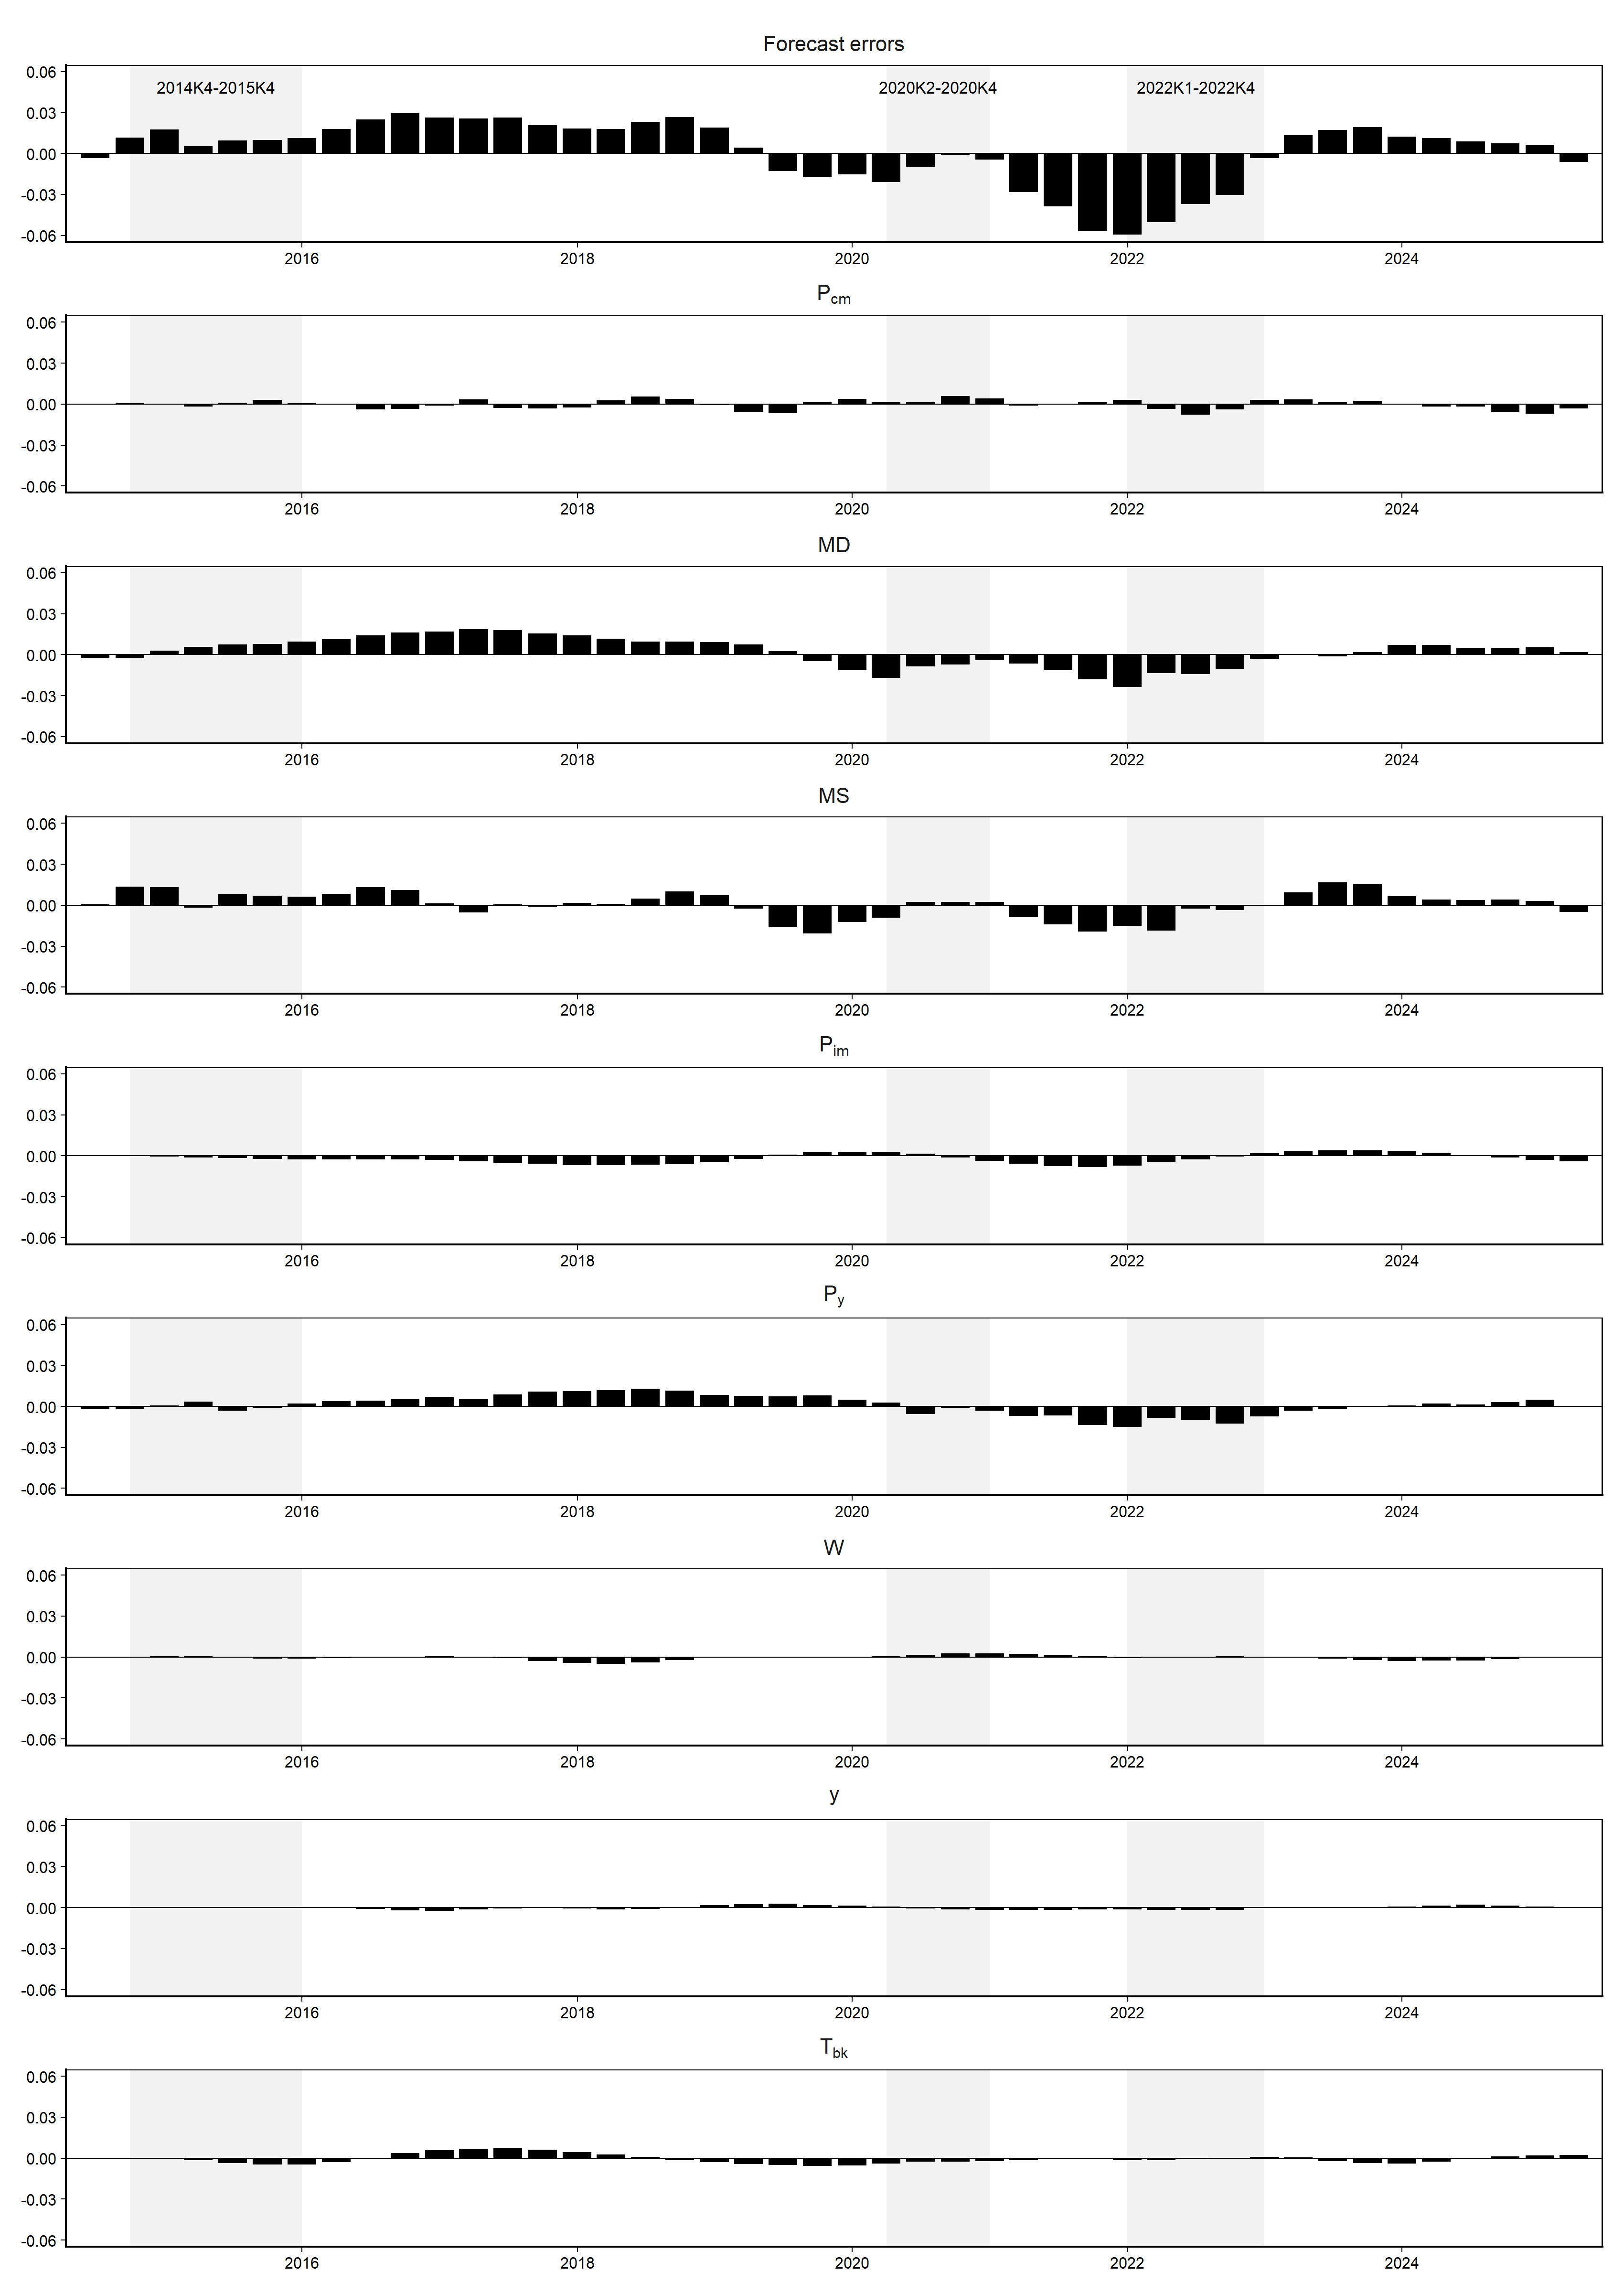
\includegraphics[
    width=\textwidth,
    height=0.84\textheight,
    keepaspectratio
]{historical_decomposition_m2.png}
\end{frame}

\begin{frame}[t,noframenumbering]{Приложение: историческая декомпозиция $R$}
\vspace{-0.25cm}
\centering
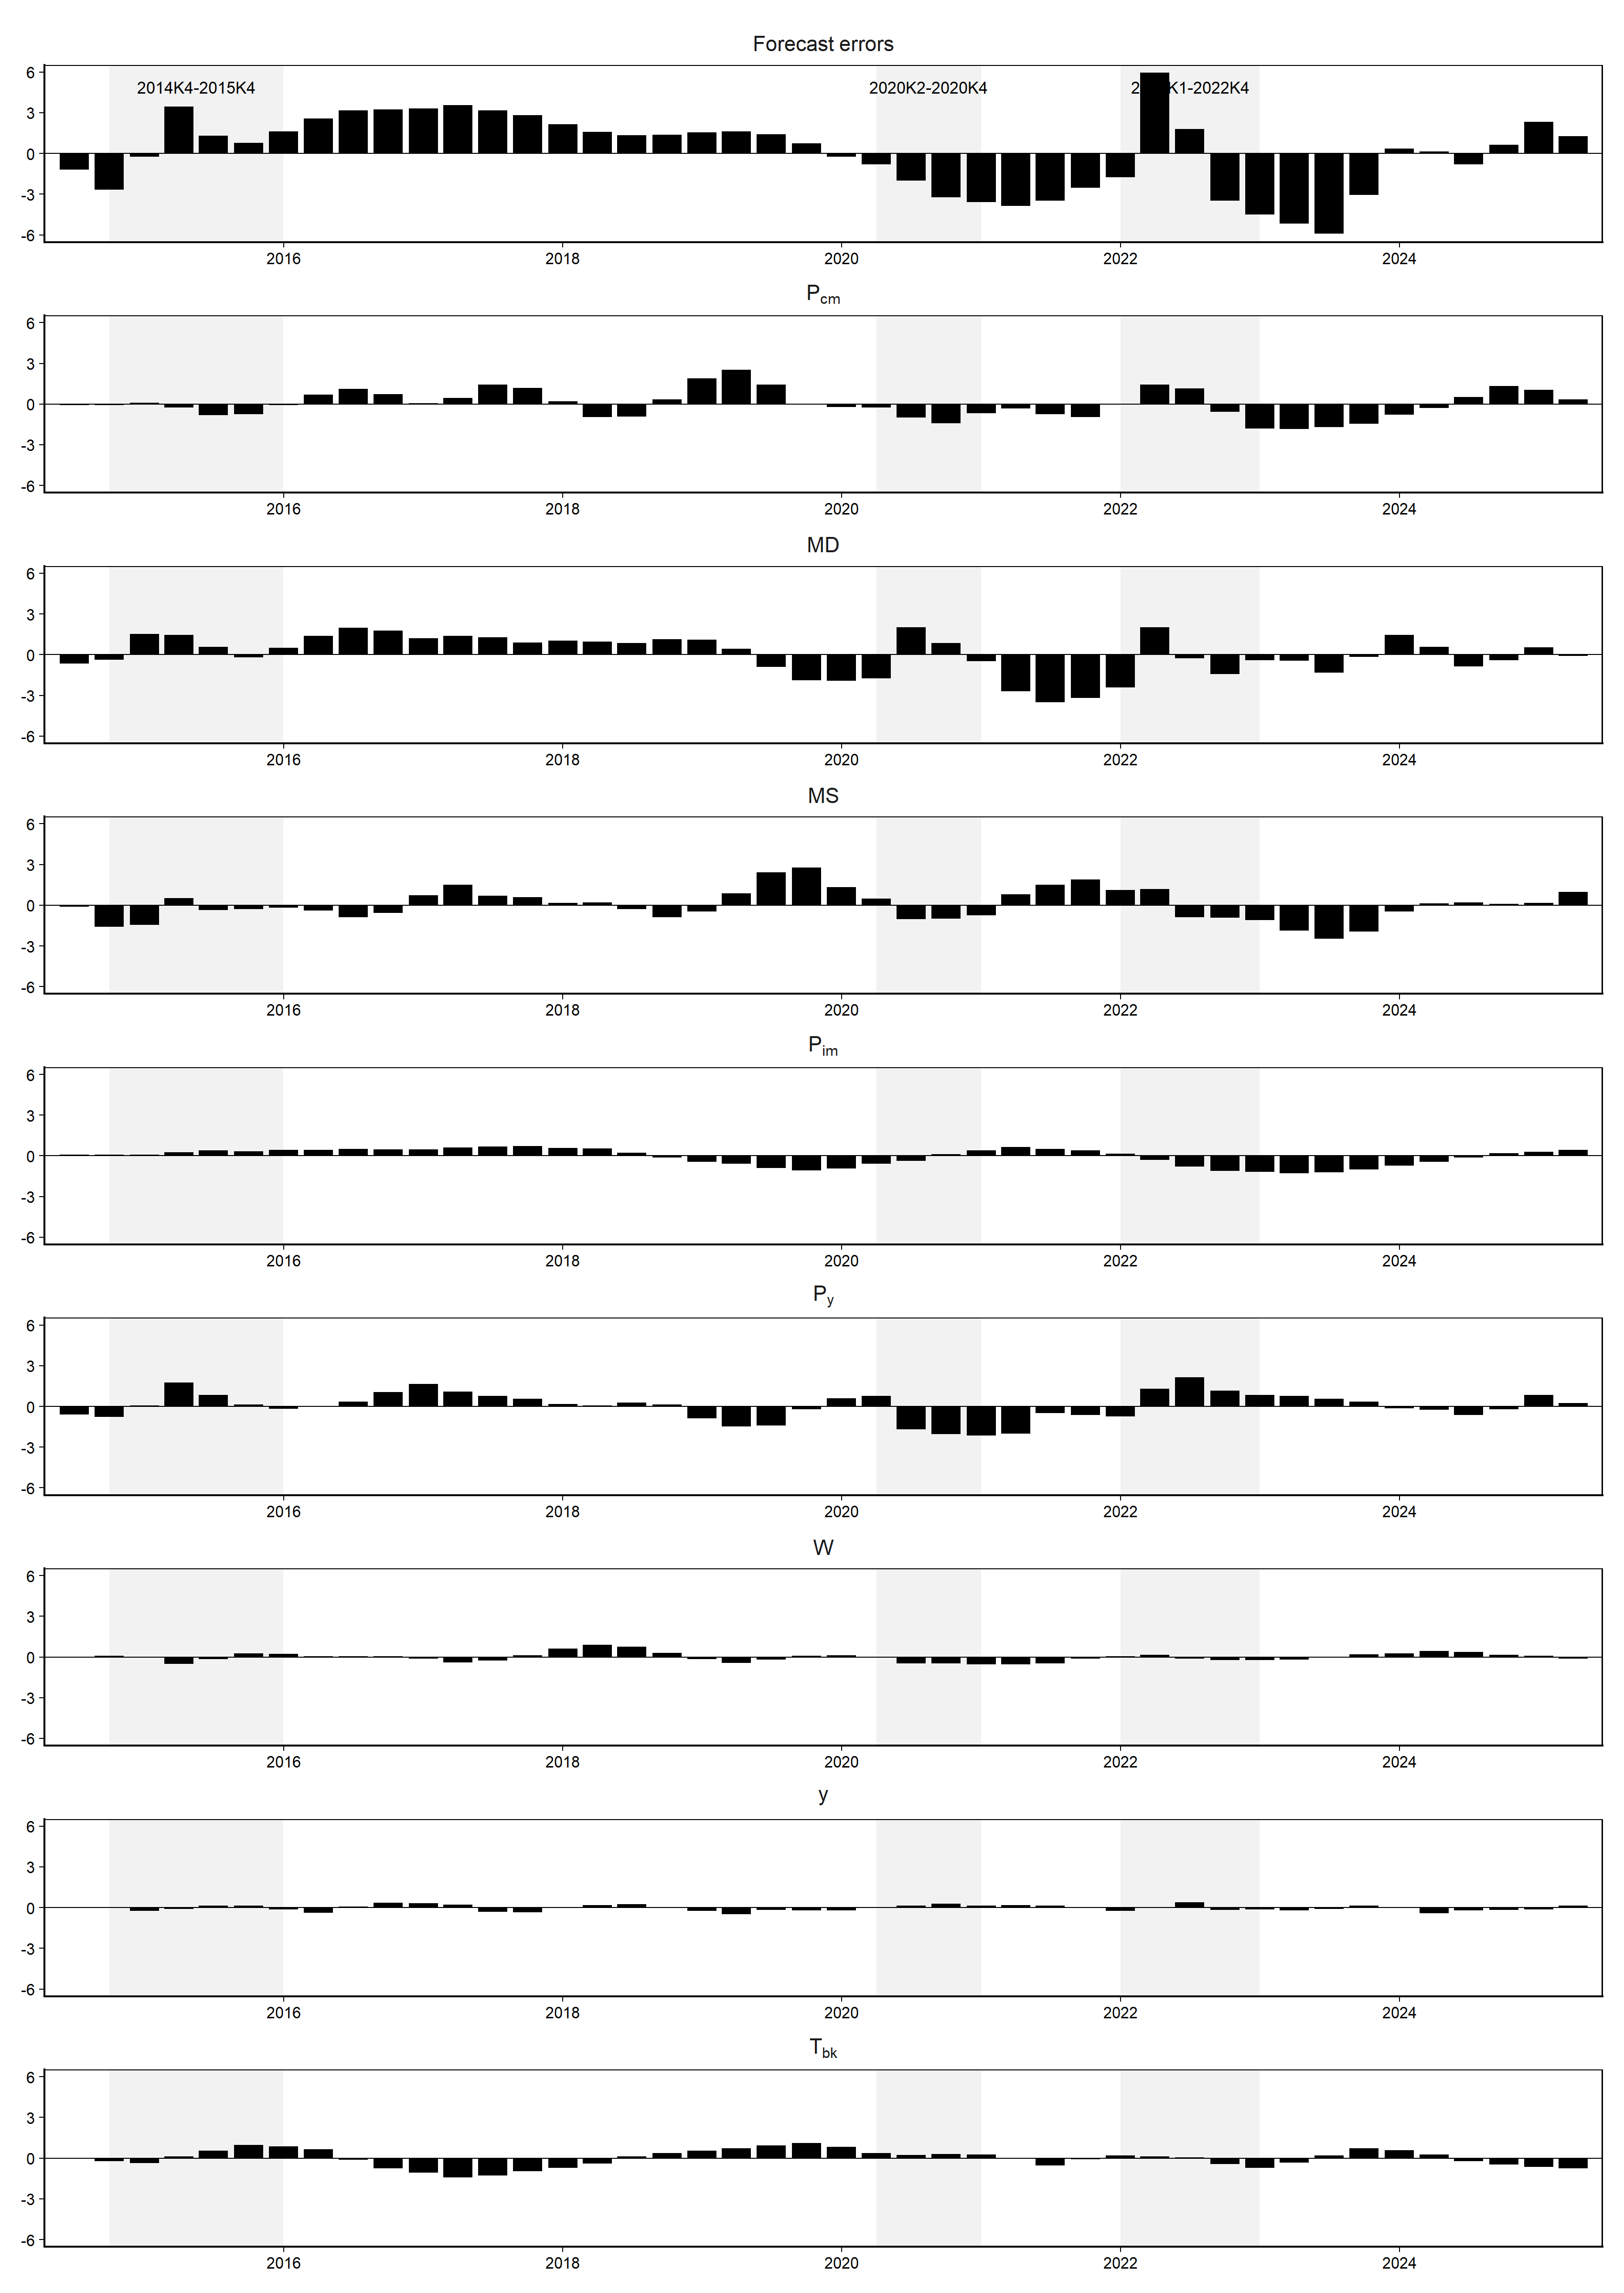
\includegraphics[
    width=\textwidth,
    height=0.84\textheight,
    keepaspectratio
]{historical_decomposition_key_rate.png}
\end{frame}

\begin{frame}[t,noframenumbering]{Приложение: историческая декомпозиция $P_y$}
\vspace{-0.25cm}
\centering
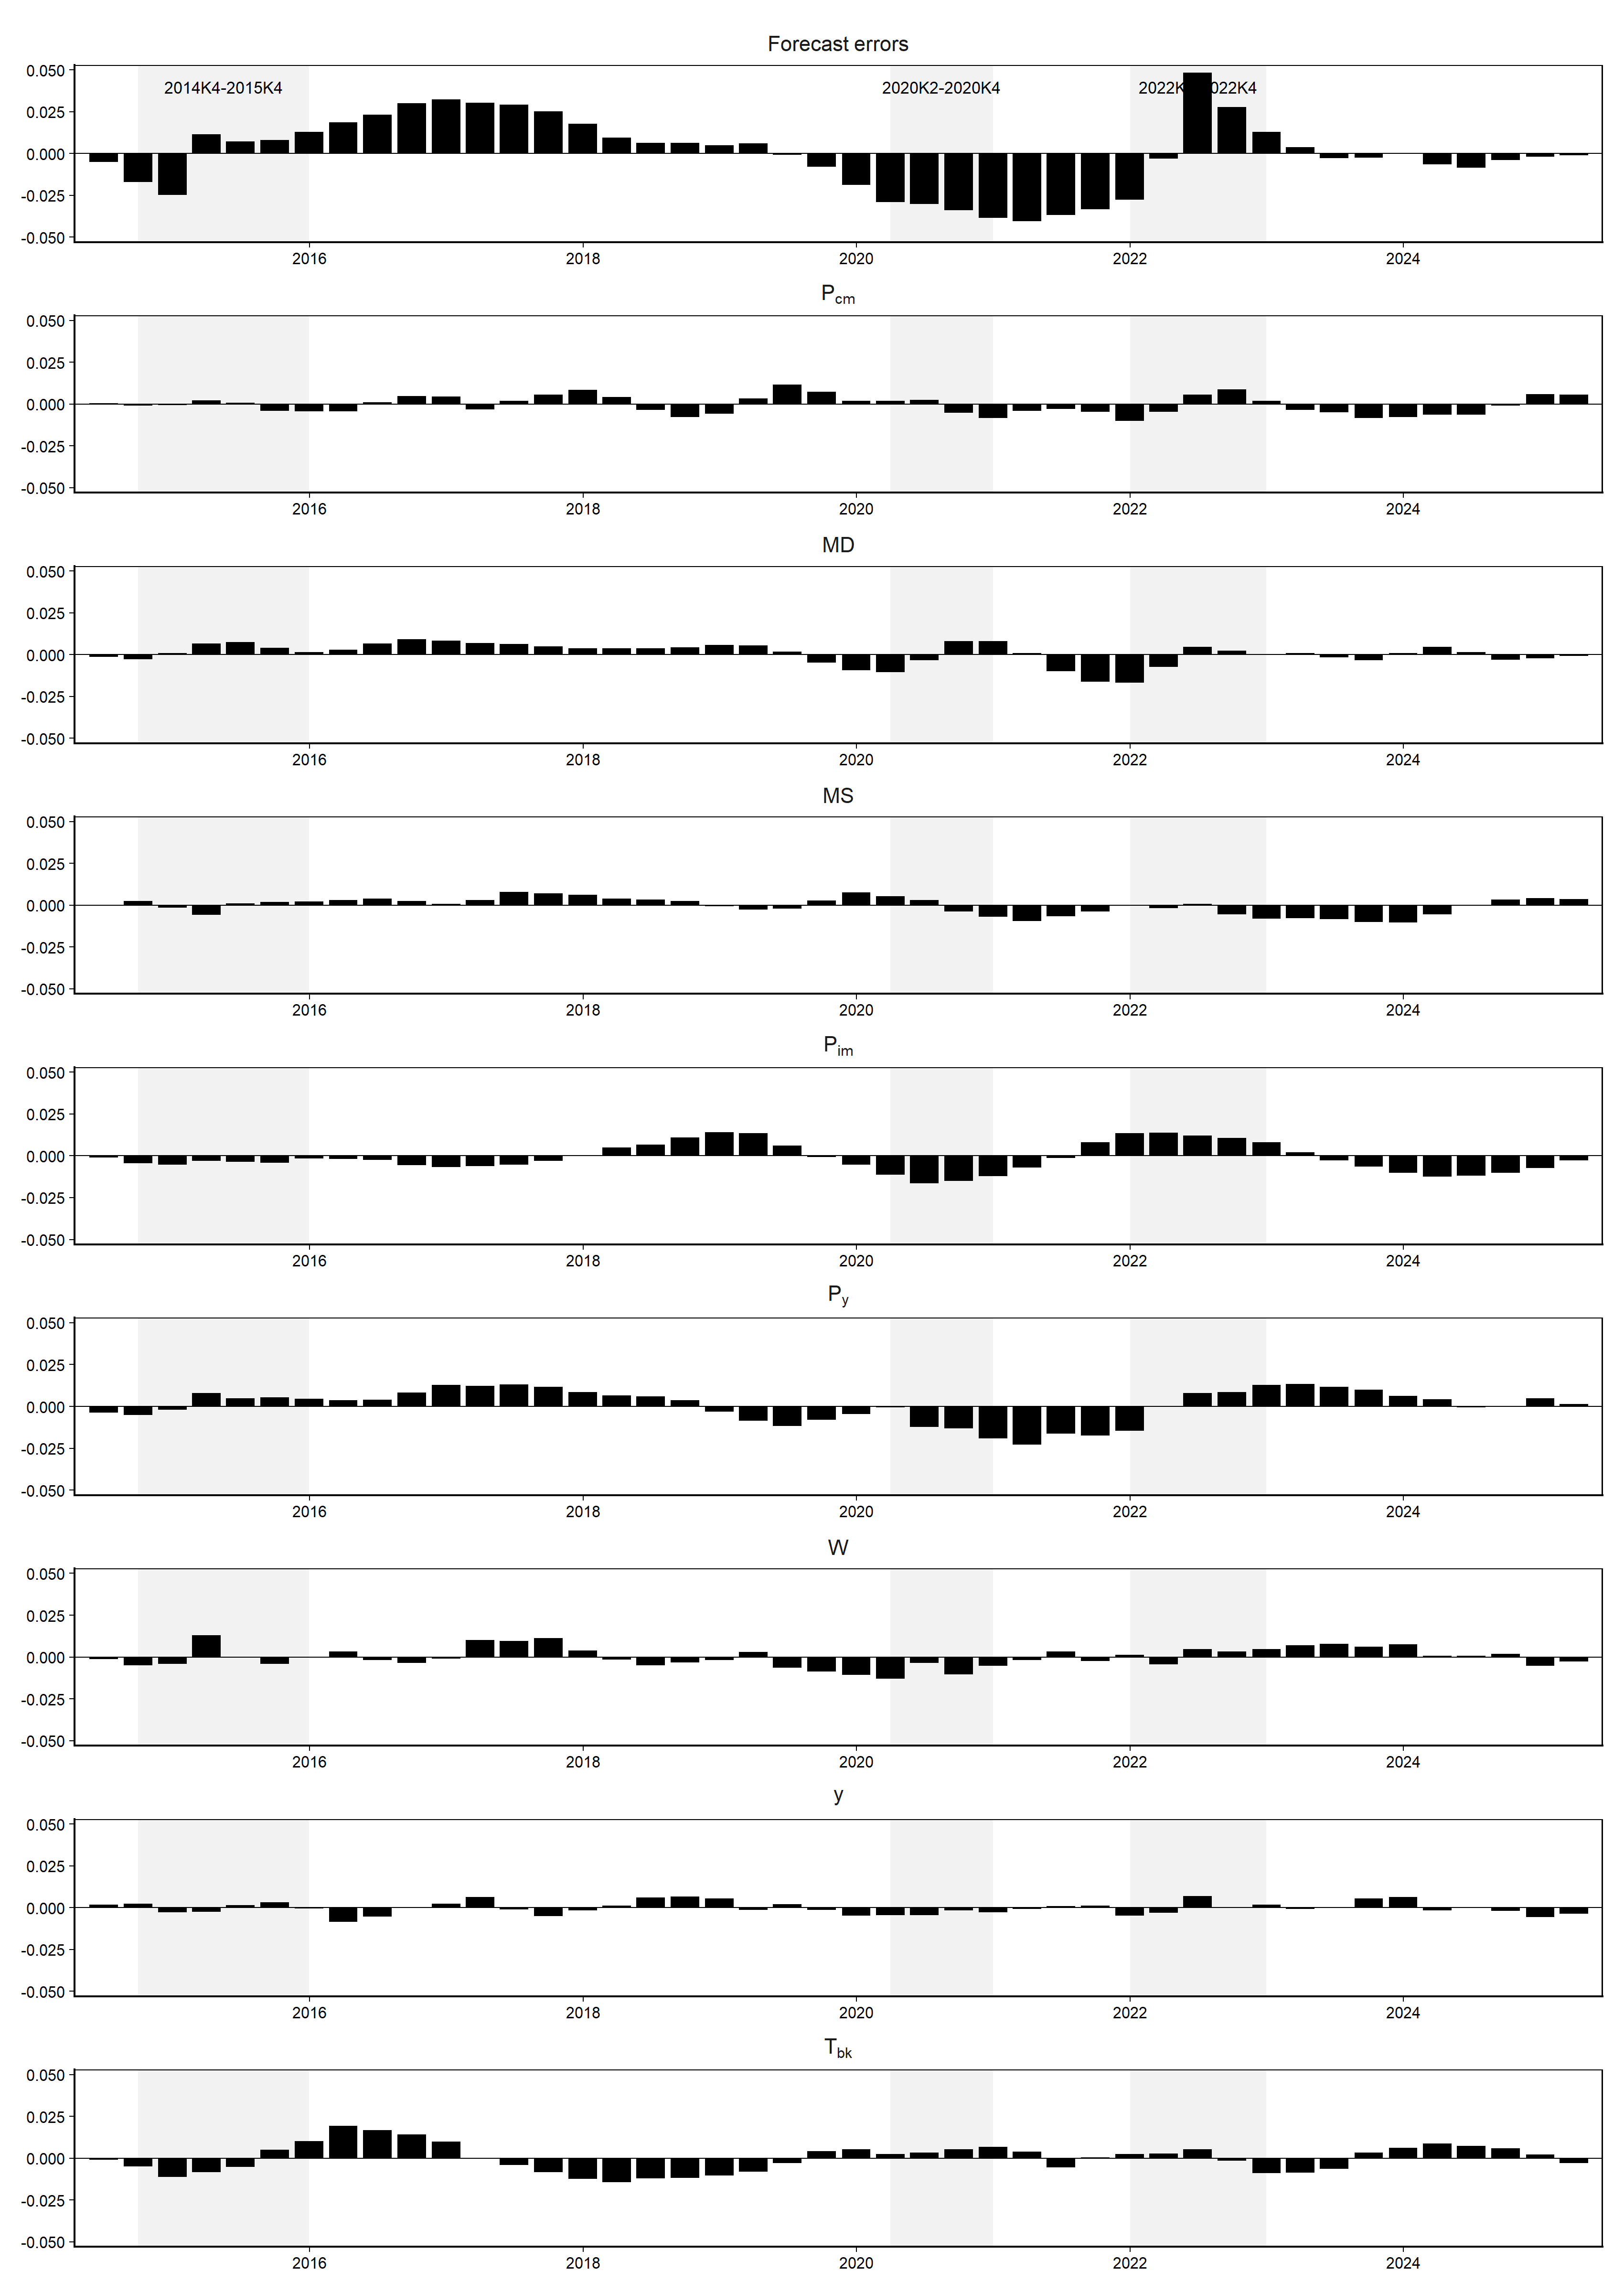
\includegraphics[
    width=\textwidth,
    height=0.84\textheight,
    keepaspectratio
]{historical_decomposition_cpi.png}
\end{frame}

\begin{frame}[t,noframenumbering]{Приложение: историческая декомпозиция $y$}
\vspace{-0.25cm}
\centering
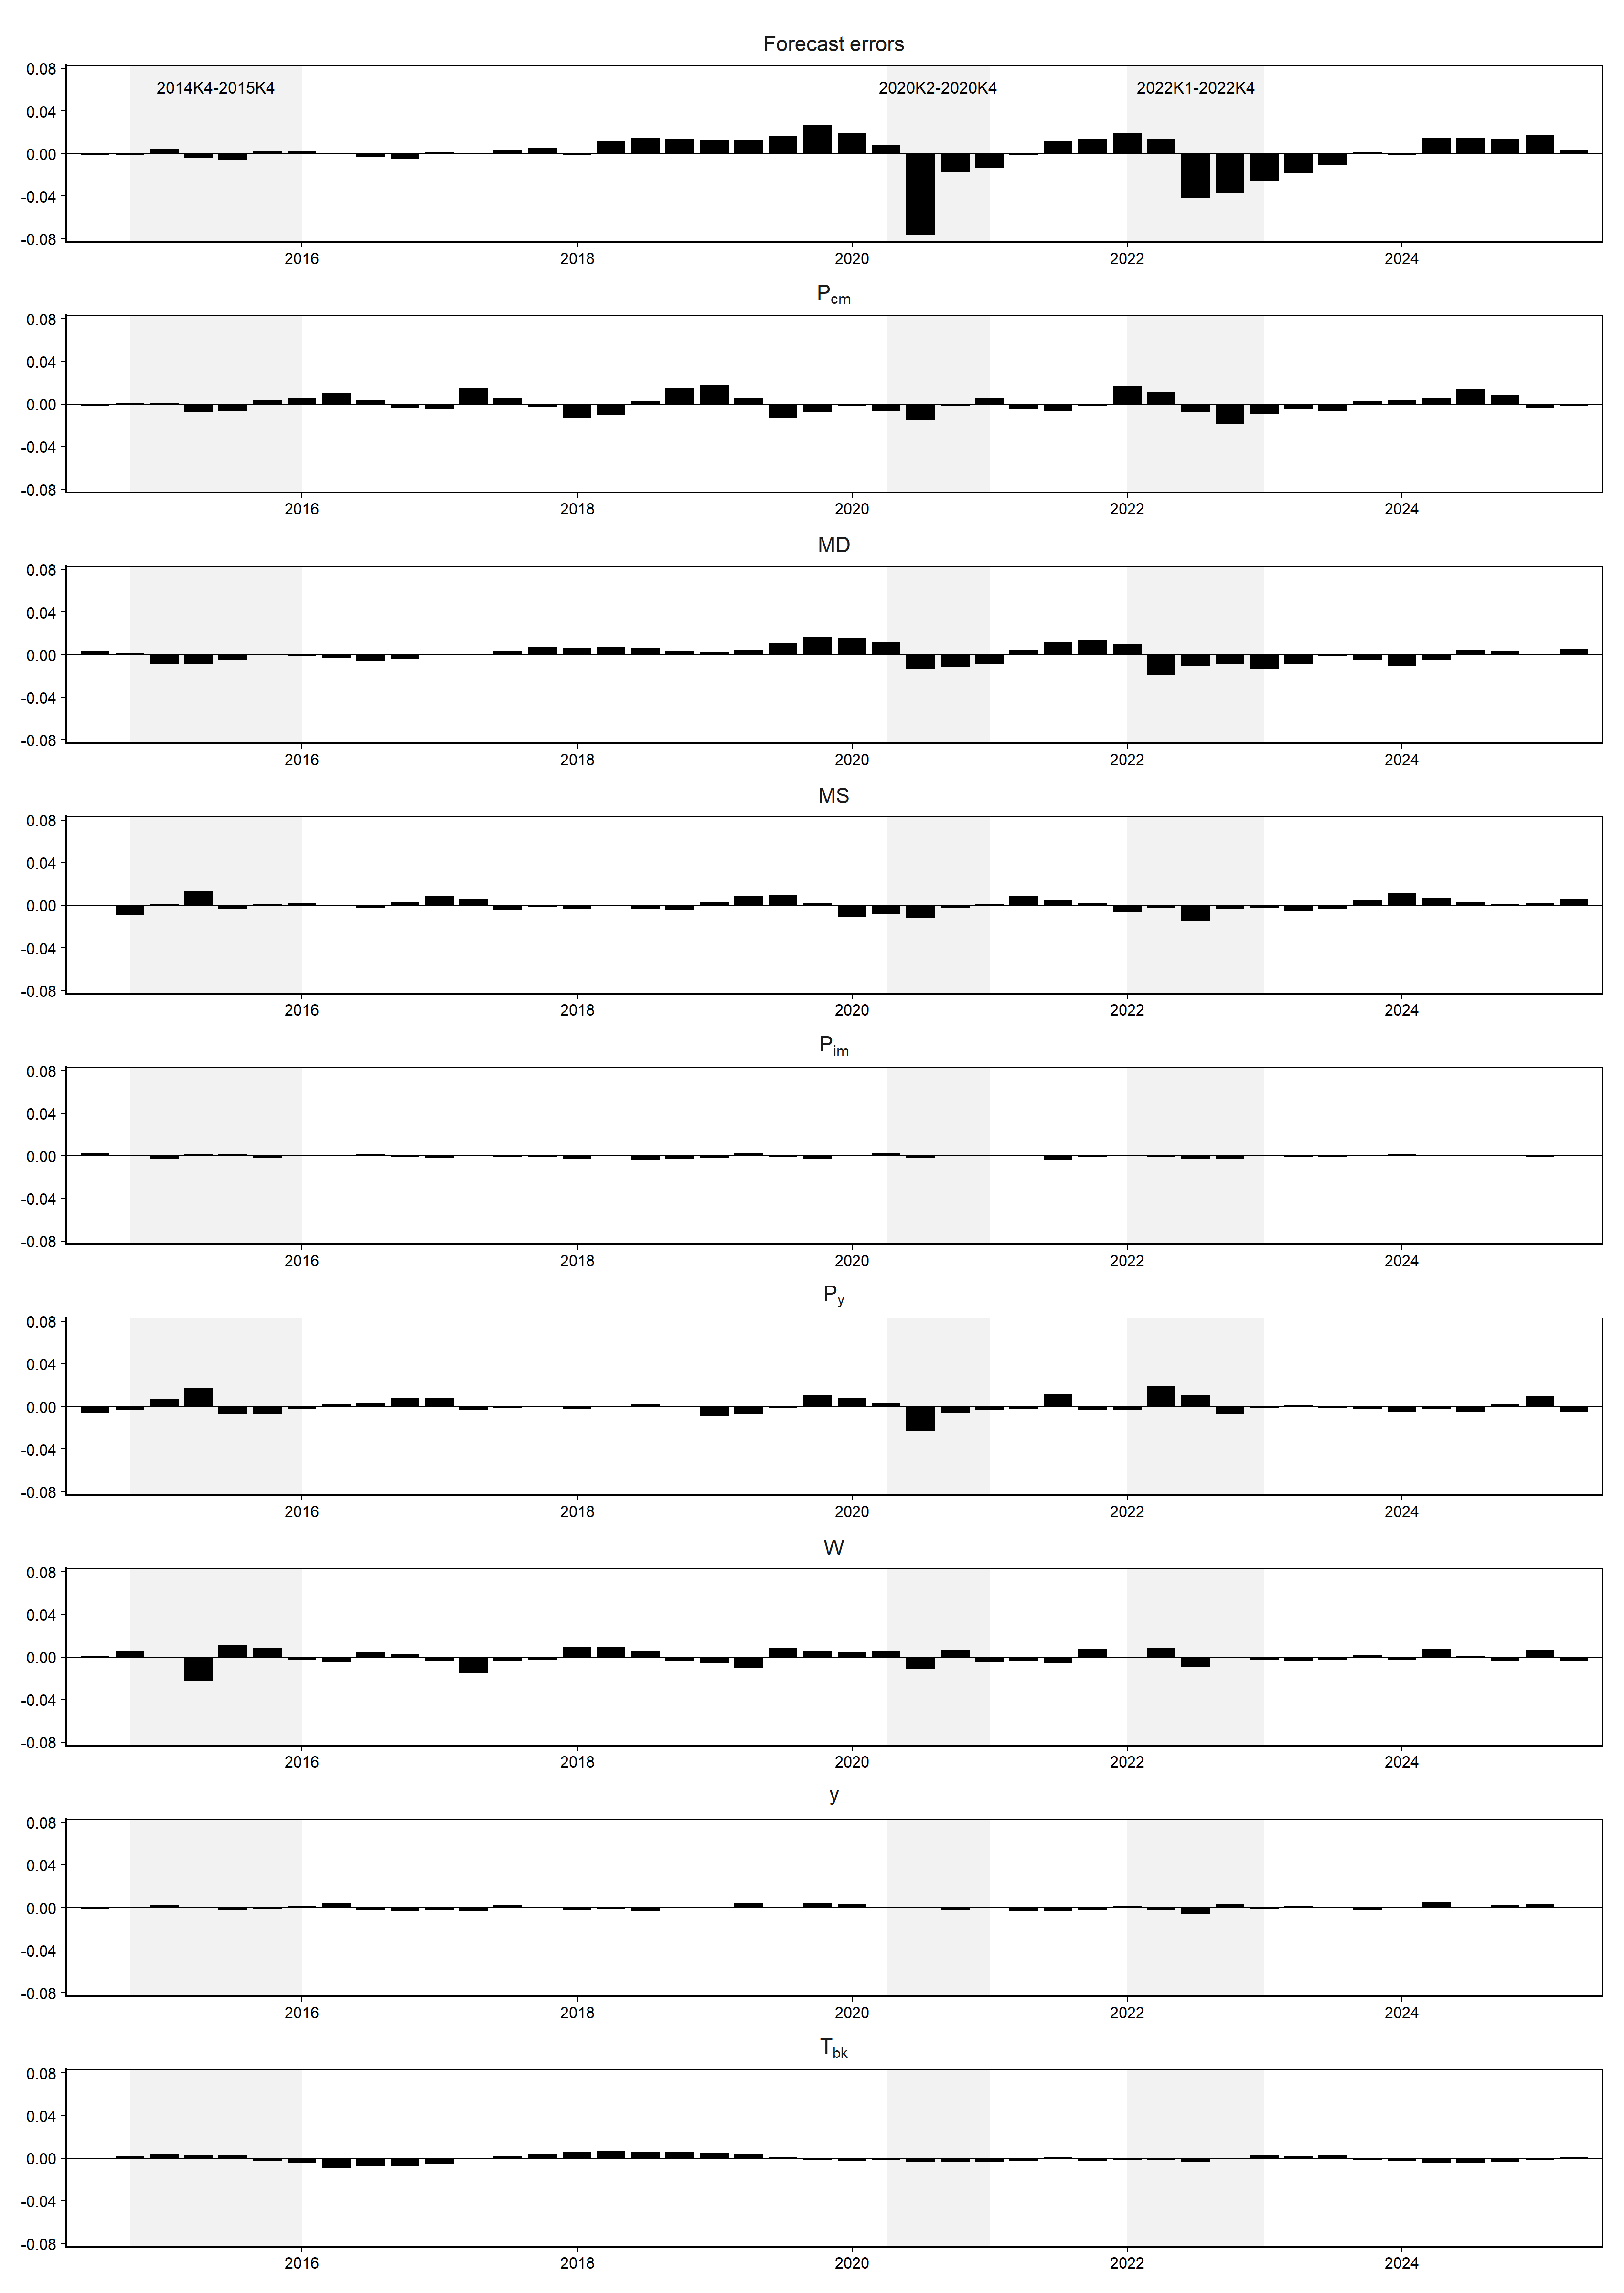
\includegraphics[
    width=\textwidth,
    height=0.84\textheight,
    keepaspectratio
]{historical_decomposition_gdp.png}
\end{frame}

\begin{frame}[t,noframenumbering]{Приложение: структурные шоки, часть 1}
\vspace{-0.25cm}
\centering
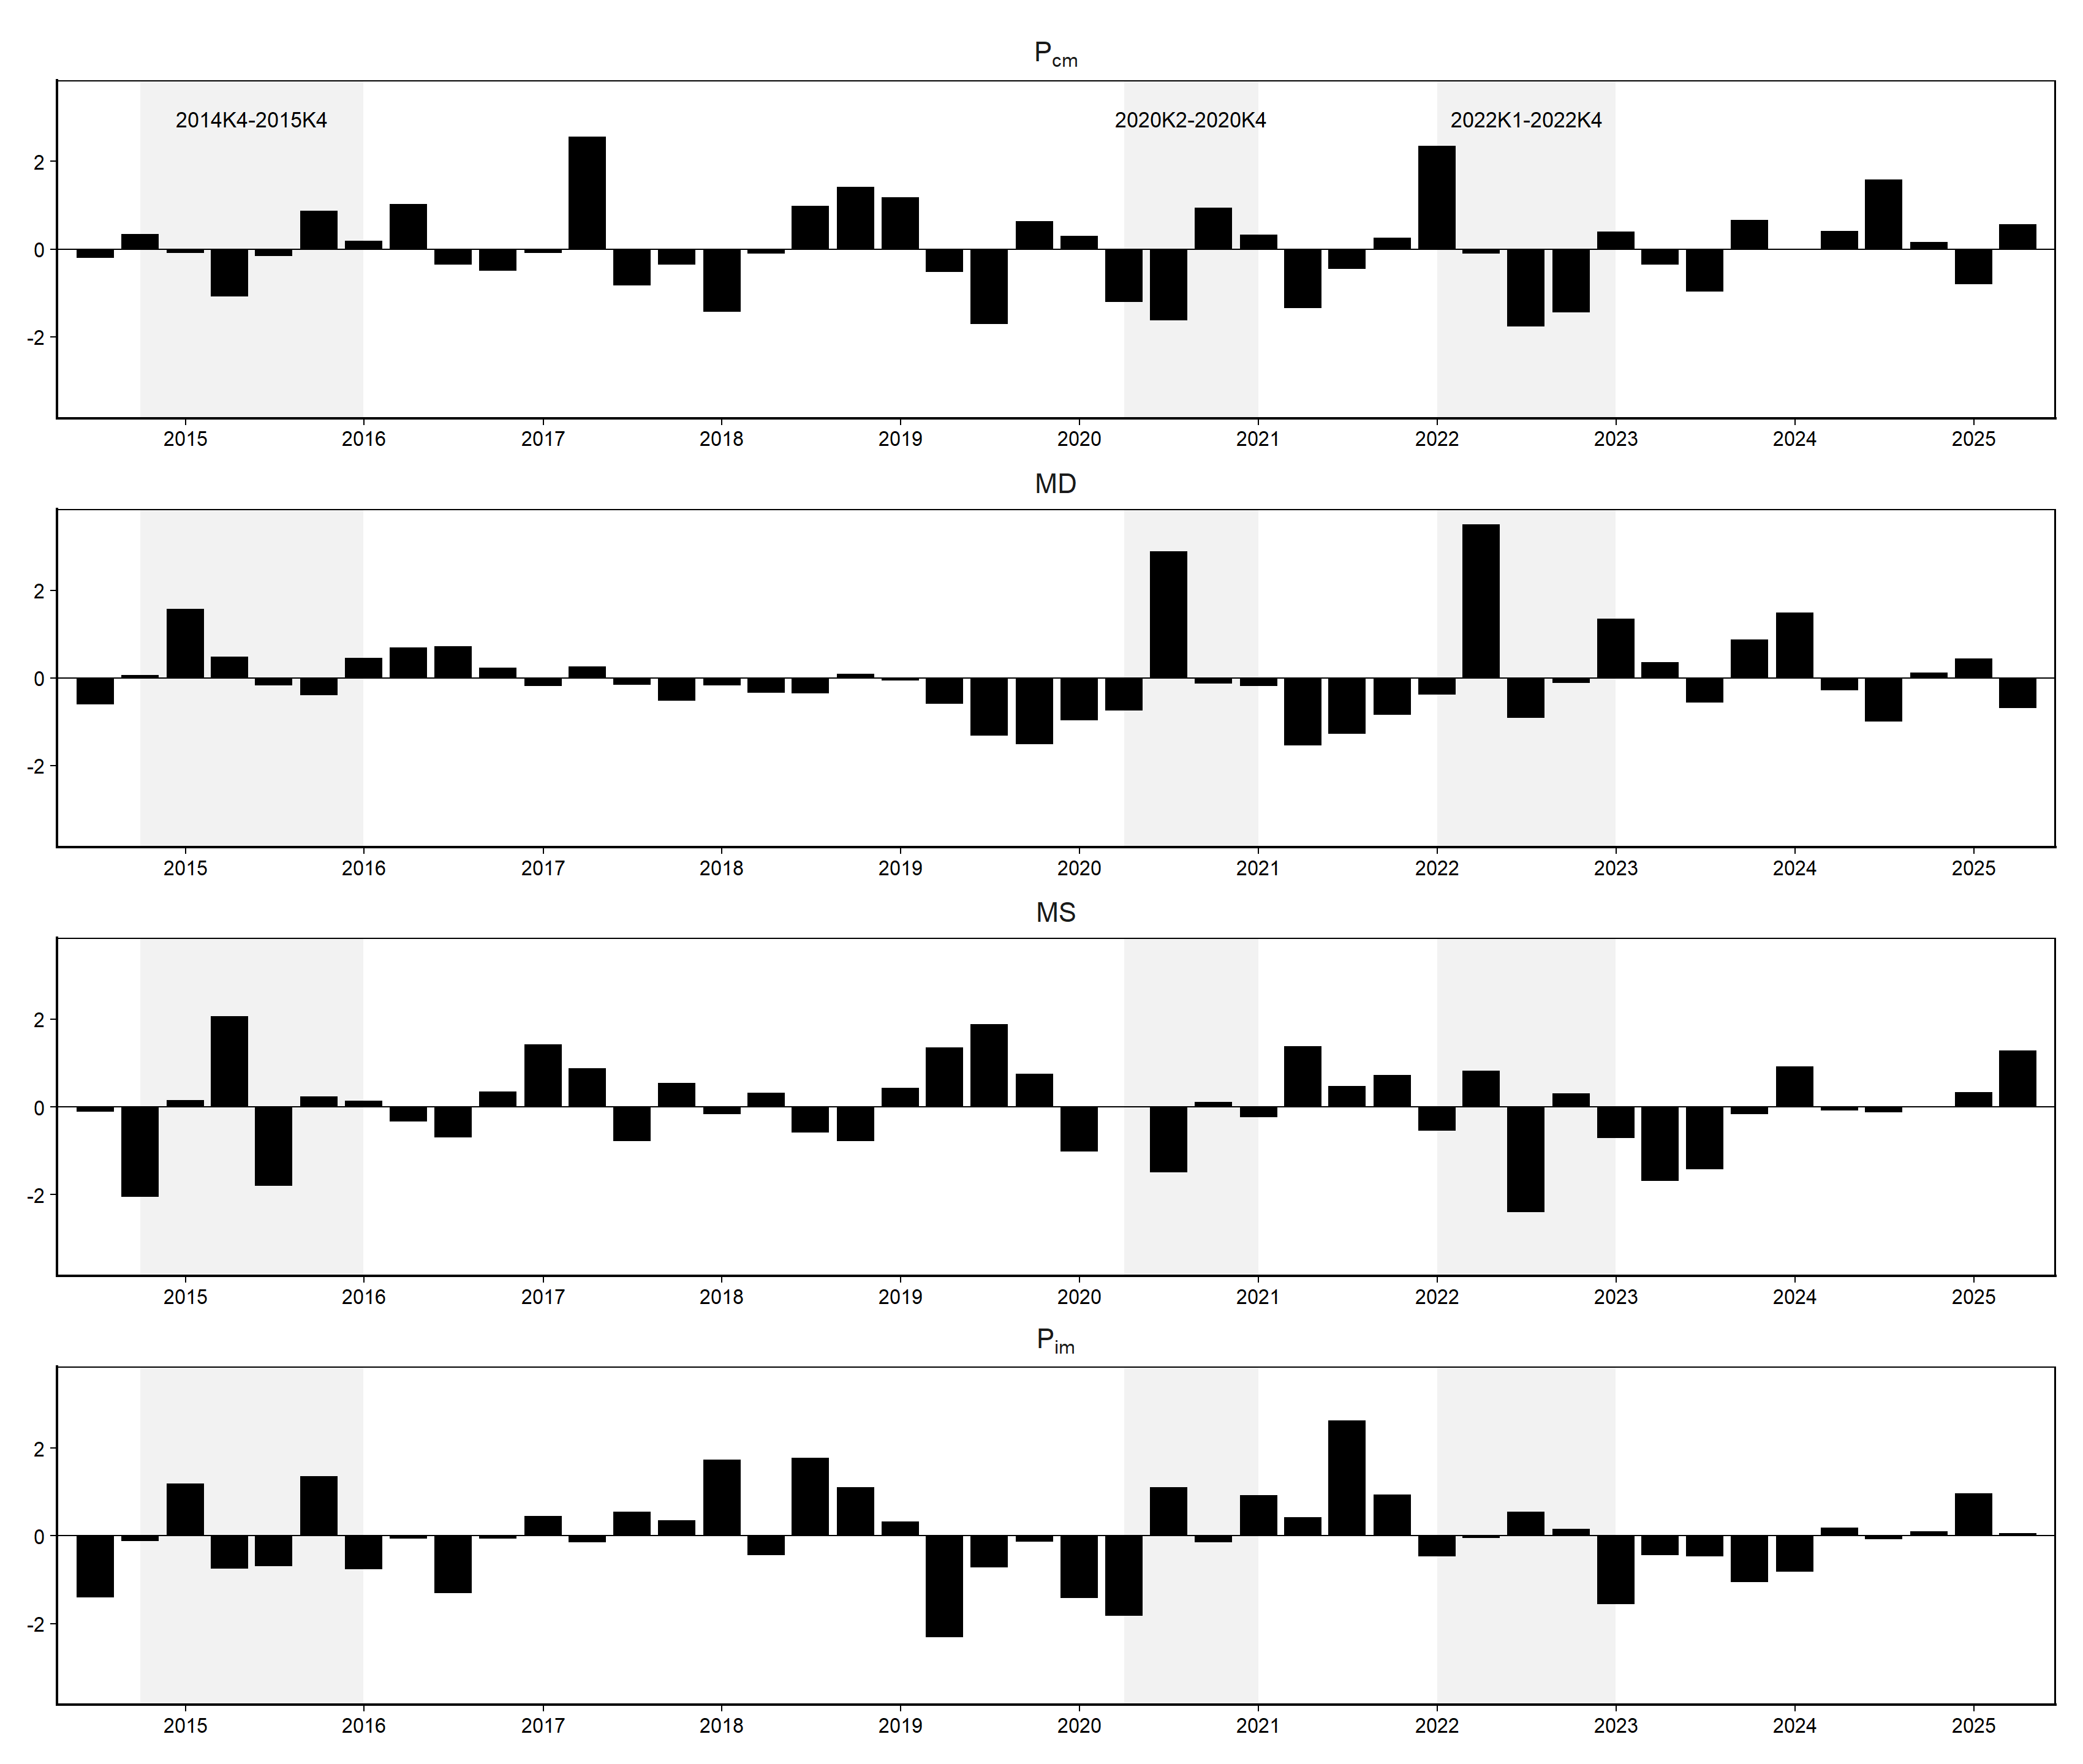
\includegraphics[
    width=\textwidth,
    height=0.84\textheight,
    keepaspectratio
]{structural_shocks_8a.png}
\end{frame}

\begin{frame}[t,noframenumbering]{Приложение: структурные шоки, часть 2}
\vspace{-0.25cm}
\centering
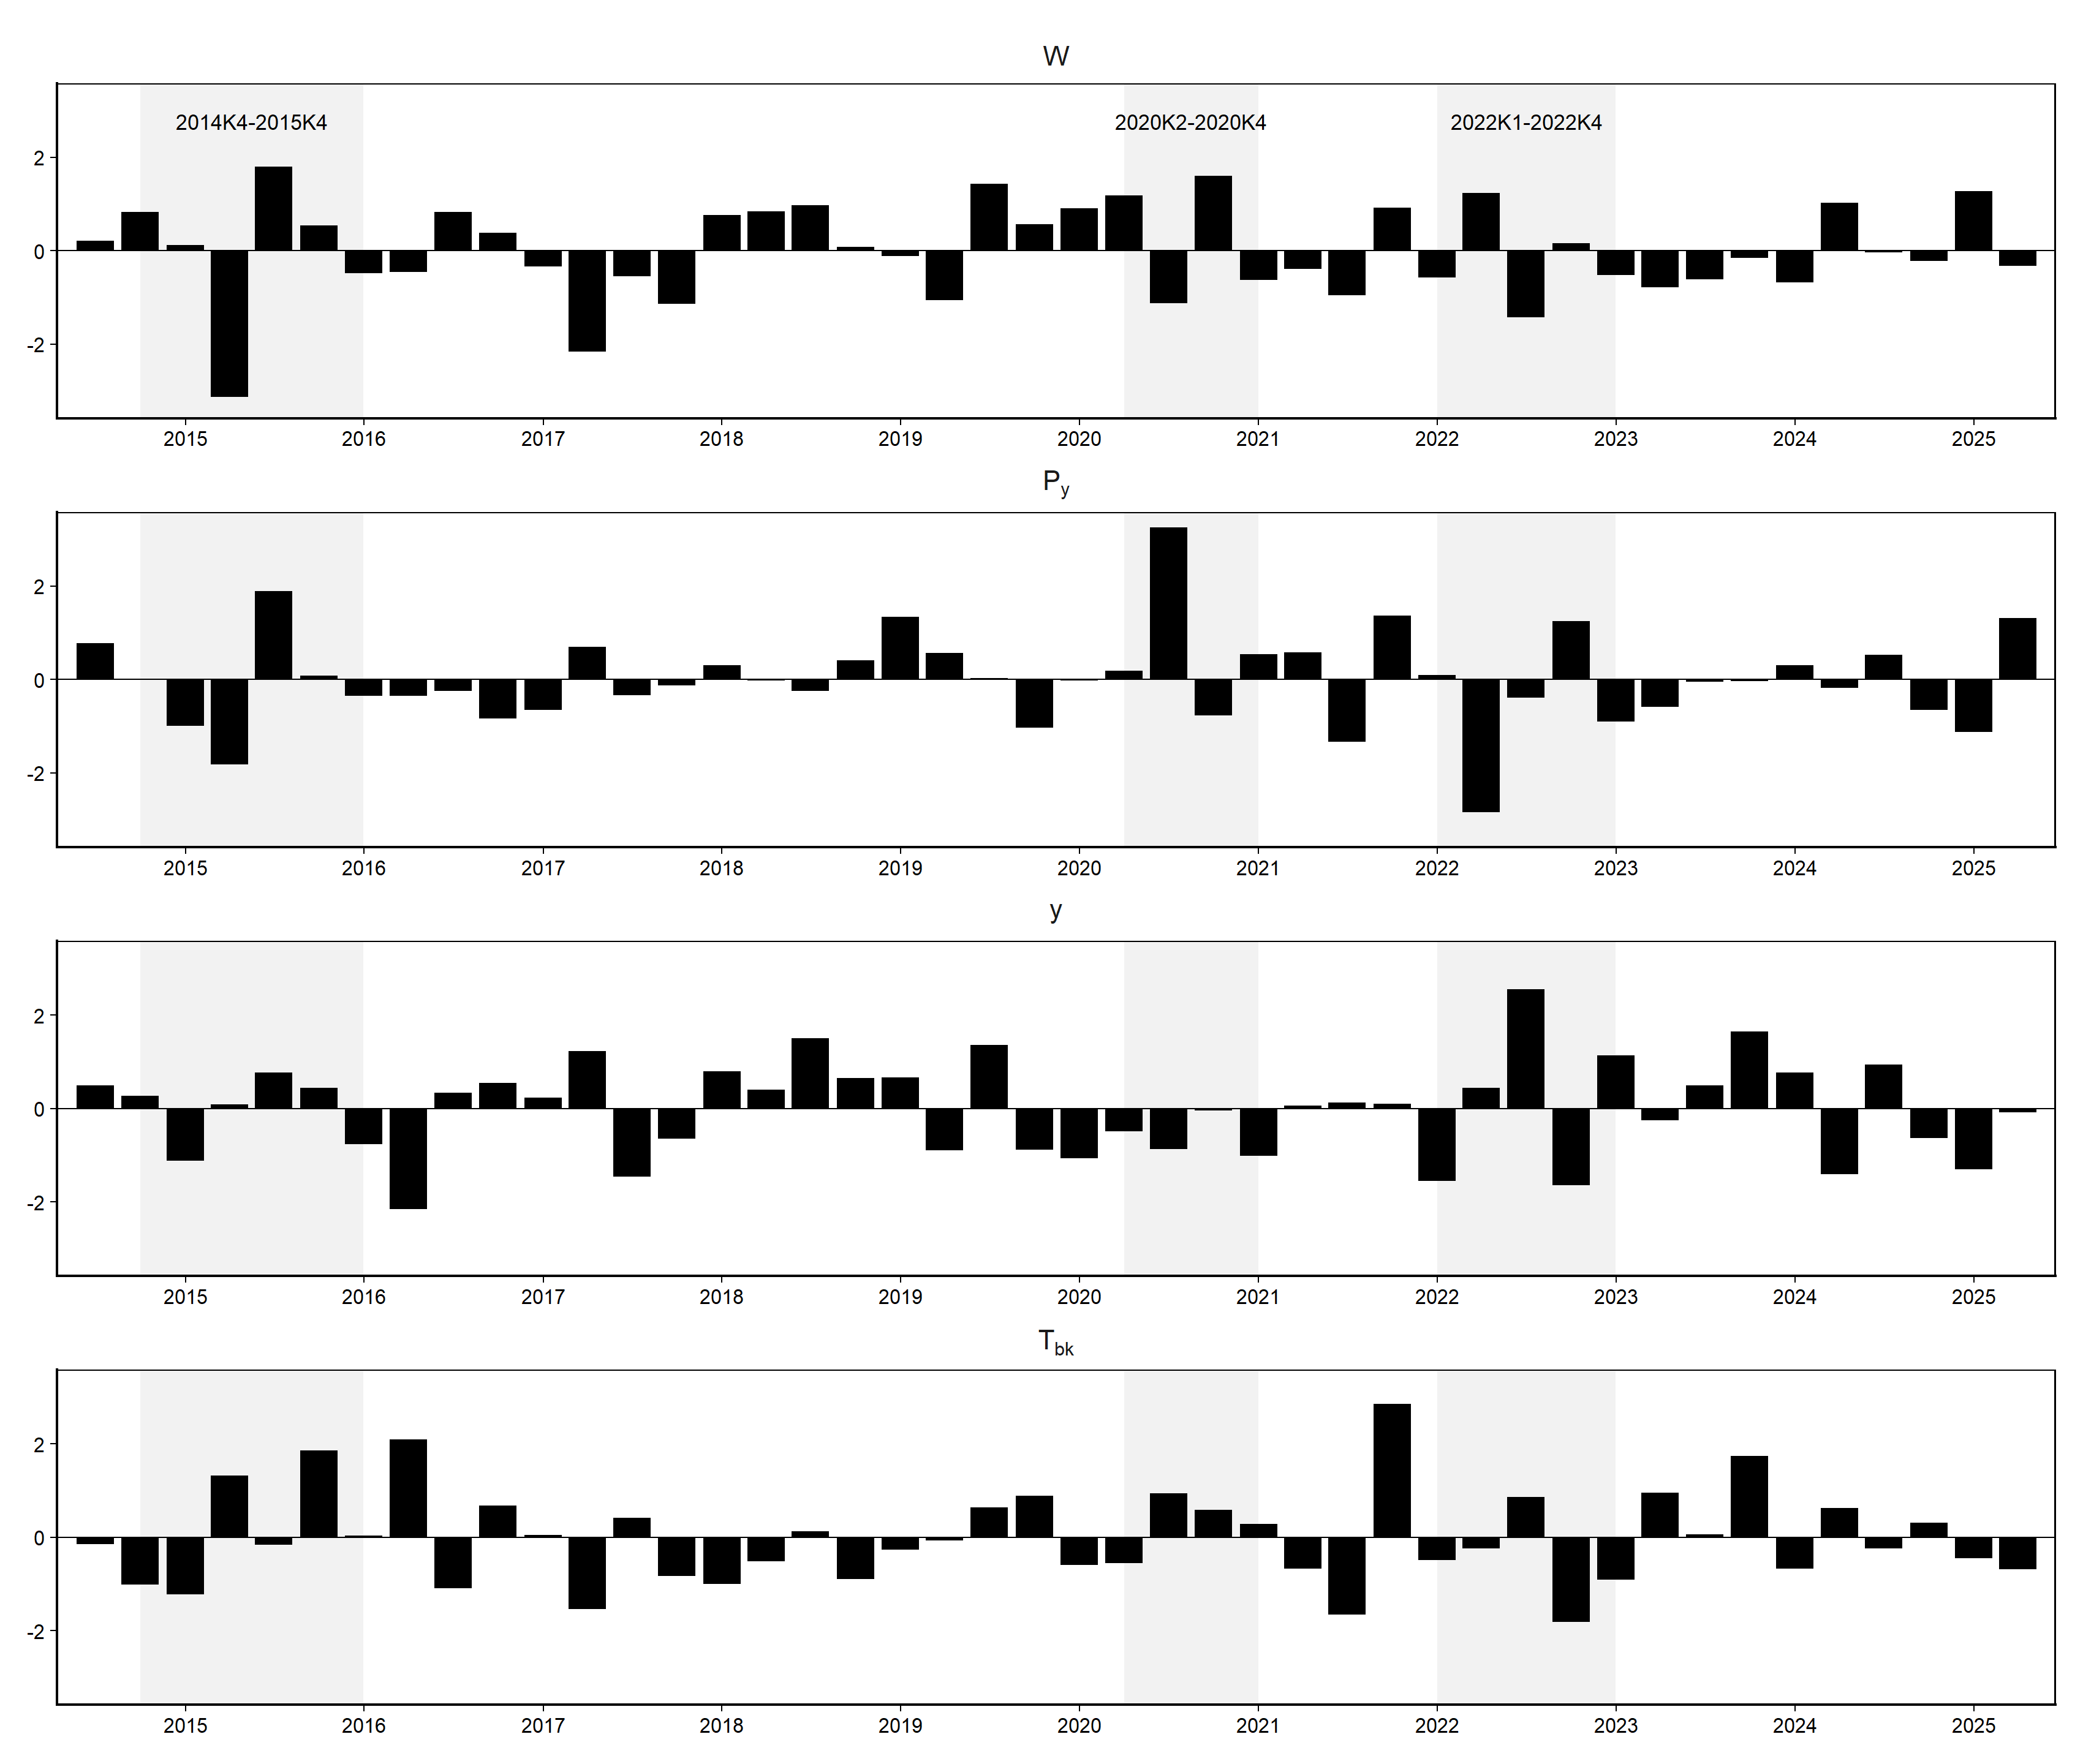
\includegraphics[
    width=\textwidth,
    height=0.84\textheight,
    keepaspectratio
]{structural_shocks_8b.png}
\end{frame}

% \begin{frame}[t,noframenumbering]{Приложение: спецификация VAR/SVAR}
% \vspace{-0.15cm}
% \centering
% \scriptsize
% \setlength{\tabcolsep}{4pt}
% \renewcommand{\arraystretch}{0.95}
% \begin{tabular}{ll}
\toprule
item & value\\
\midrule
frequency & quarterly\\
sample period & 2014Q1--2025Q1\\
observations after lags & 44\\
lag order & p = 1\\
variables & Pcm, M2, R, Pim, Py, W, y, OvDeb\\
\addlinespace
transformations & log-levels for level variables; R without log\\
model type & VAR(1) / SVAR(1)\\
\bottomrule
\end{tabular}

% \end{frame}

\begin{frame}[t,noframenumbering]{Приложение: информационные коэффициенты}
\vspace{-0.15cm}
\centering
\scriptsize
\setlength{\tabcolsep}{4pt}
\renewcommand{\arraystretch}{0.95}
\begin{tabular}{rrrrr}
\toprule
lag & AIC & HQ & SC & FPE\\
\midrule
1 & -54.282 & -53.177 & -51.147 & 0.000\\
2 & -54.542 & -52.455 & -48.621 & 0.000\\
3 & -57.754 & -54.684 & -49.046 & 0.000\\
4 & -200.140 & -196.088 & -188.646 & 0.000\\
5 & Inf & Inf & Inf & 0.000\\
\addlinespace
6 & Inf & Inf & Inf & 0.000\\
7 & Inf & Inf & Inf & 0.000\\
8 & Inf & Inf & Inf & 0.000\\
\bottomrule
\end{tabular}

\end{frame}

\begin{frame}[t,noframenumbering]{Приложение: устойчивость VAR}
\vspace{-0.15cm}
\centering
\scriptsize
\setlength{\tabcolsep}{6pt}
\renewcommand{\arraystretch}{0.95}
\begin{tabular}{lr}
\toprule
root\_id & modulus\\
\midrule
1 & 1.018\\
2 & 0.985\\
3 & 0.751\\
4 & 0.751\\
5 & 0.659\\
\addlinespace
6 & 0.659\\
7 & 0.451\\
8 & 0.451\\
stable & FALSE\\
\bottomrule
\end{tabular}

\end{frame}


}
\end{document}
